%%%%%%%%%%%%%%%%%%%%%%%%%%%%%%%%%%%%%%%%%%%
%THIS FILE CONTAINS ALL COMMON COMMANDS NEEDED FOR COMPILATION INTO BOTH PDF AND HTML.
%THE EXTENSION file src/macros.sty CONTAINS ONLY COMMANDS NEEDED EXCLUSIVELY FOR COMPILATION INTO PDF
%THE DIRECTORY src/hva/ CONTAINS ONLY COMMANDS NEEDED EXCLUSIVELY FOR COMPILATION INTO HTML WITH HEVEA, WITH THREE EXTENSION FILES, imakeidx.hva, macros.hva AND picins.hva.
%%%%%%%%%%%%%%%%%%%%%%%%%%%%%%%%%%%%%%%%%%%
% 2024/04:
% - \documentclass[] : change {book} to {scrbook} from KOMA-script -> rewritting the manual.
% - change fancyhdr to scrlayer-fancyhdr (compatibility with scrbook) to scrlayer-scrpage (contained in koma-script) -> modify macros.sty too.
% - rewriting title page for \maketitle (use with pandoc [produce html file], \begin(title)...\end(title) doesn't work with pandoc, "microtype" package too)
% 2024/10
% - renaming chapter files with an order number
% - clean documentclass / packages / add comments
% 2024/10
% - comment \ifIllustration to always have pictures in manuel
% - texlive-extra-utils -> make4ht
% 2024/11
% - simplification of \usepackage{graphicx} when pdf

%\ifx\pdfoutput\undefined		% if no pdfLaTeX outputting
% test KOMA-script with "scrbook" instead of "book"
%\documentclass[%
%	paper=a4,			% default=a4 and therefore not needed
%	12pt,				% default=11pt
%	headsepline,		% line under the header
%	footsepline,		% line above the footer
%	twoside=semi		% same left/right margins, default=twoside
%]{scrbook} 			% 
%}{
%\else							% else pdfLaTeX outputting
\documentclass[%
%	pdflatex,			% commented to avoid compilation errors
	a4paper,			% default=a4 and therefore not needed
	12pt,				% default=11pt
	english,			% use in babel, translator and varioref packages options %TODO: change with ngerman/english option in de/en manuals
	toc=listof,			% add a "lof" (list of figures) line at the begining of the toc (table of contents)
	twoside=semi,		% same recto/verso margins similar to simple verso margins, default=twoside
	open=any,			% avoids the empty right/even page between chapters
	headsepline,		% draw rule below header
	footsepline,		% draw rule above footer
	plainfootsepline 	% draw footsepline on plain pages (here for heading pages, may be due to twoside=semi in scrbook options
]{scrbook} 				% KOMA-Script class "book"		
%}
%\fi

%\usepackage{ifpdf}					% detect pdfTeX, replaced by \Ifpdfoutput (KOMA-script)
\usepackage[T1]{fontenc}			% the font encoding
%\usepackage[utf8]{inputenc}			% no longer need to specify, included in LaTex since April 2018
\usepackage{lmodern}				% Latin Modern police
\usepackage{babel}					% use the language define in \documentclass
%\def\frenchcontentsname{Sommaire}	% rename "Table des matières" (at end of document) from [french]{babel} to "Sommaire" (at start of document)
%\frenchsetup{ItemLabeli=\textbullet}	% change 1st level list marker of french babel
%\frenchsetup{ItemLabelii=-}			% change 2nd level list marker of french babel
\usepackage{enumitem}				% control layout of itemize and enumerate lists
\usepackage{translator}		% for translating the Fixed Names
\usepackage{textcomp}				% for special characters like \textcurrency
%\usepackage{txfonts}
%\usepackage{ae}
%\usepackage{cmbright}
%\usepackage{times}					% changed from txfonts
\usepackage{newtxtext}				% install texlive-fonts-extra, replacing times which replaces txfonts
%\usepackage{lwarp}					% produce html file with lwarp (install texlive-extra-utils)

\usepackage[letterspace=300]{microtype}		% Font expansion (use for title) with "lsstyle" (and "\textls[x] which doesn't work with pandoc) / espace entre caractères (utilisé pour le titre)
% Web addresses
%\usepackage{url}					% loaded by hyperref


% --------------------------------------------
% Load graphicx package with pdf if needed
% --------------------------------------------
%\ifpdf
%%\Ifpdfoutput{%
	%%\usepackage[pdftex]{graphicx}		% enhanced support for importing graphics (x=enhanced) and then using the \includegraphics command to insert the file
	%%}{%			
	% else								% Commented out to avoid errors in html, and put in the macros.sty file for pdf
\usepackage{graphicx}				% enhanced support for importing graphics (x=enhanced) and then using the \includegraphics command to insert the file
\newcommand{\refimage}[1]{ (fig. \vref{#1})}	% for the hypertext link display on images
\newcommand{\vspacepdf}[1]{\vspace{#1}}			% for spaces after images bordered with text
	%%}
%% Graphics Extensions
%\ifpdf
%%\Ifpdfoutput{%
	%%\DeclareGraphicsExtensions{.pdf,.png,.jpg}
	%%}{%
	%\else
	%%\DeclareGraphicsExtensions{.eps}
	%%}
%\fi


% For illustrations
%\usepackage{picins}				% for text around image TODO change to wrapfig2 in the manuel
\usepackage{wrapfig2}				% TODO change in chapters, for text around image (replace picins)
\usepackage{caption}				% for good references in table of figures


%\usepackage{scrlayer-fancyhdr}		% facilities for constructing headers and footers, replace fancyhdr
% change to scrlayer-scrpage here and in macros.sty


%\pagestyle{fancyplain}
%\usepackage{tabularx}
%\usepackage{hhline}				% produce single or double line
%\usepackage{layout}				% TODO: Only if DE mode
\usepackage{varioref}		% defines the commands \vref, \vpageref, \vrefrange, and \vpagerefrange in french
%\usepackage{lastpage}
%\usepackage{longtable}
\usepackage{xcolor}					% color package improvement for several kinds of color tints, shades, tones, and mixes of arbitrary colors
%\usepackage{vmargin}				% for changing the title page margins
\usepackage{thumbpdf}				% create thumbnails (vignettes) in pdf


%\usepackage{emptypage}		% change by using \cleardoubleemptypage (in koma-scripts)
% Latex loads macros-3.0.sty for pdf output and Hevea loads /hva/macros.hva for html output
%\usepackage{macros-3.0}

%% Page layout %%
\usepackage[%
%	showframe,					% to see frame of geometry package
	top=1in,					% marge haute
	headheight=7mm,				% hauteur en-tête
	headsep=6mm,				% distance entre entête et corps de texte
	textheight=252mm,			% textheight=paperheight-topmargin-headheight-headsep-footskip
	footskip=11mm,				% distance entre bas de pied de page et bas du corps de texte
	hmargin=25mm				% horizontal margins (left and right), textwidth = paperwidt - margins
]{geometry}
\usepackage{scrlayer-scrpage}	% define and manage page styles by controlling page headers and footers			
\clearpairofpagestyles			% remove the default marks of the headings and the plain pages
\lehead{\leftmark}				% leftmark at left of even page
\lohead{\leftmark}				% leftmark at left of odd page
\rehead{\rightmark}				% rightmark at right of even page
\rohead{\rightmark}				% rightmark at right of odd page
\cfoot*{\pagemark}				% pagemark in the center of the footer
\ModifyLayer[addvoffset=-1ex]{scrheadings.foot.above.line}		% shift line up to increase distance between footer text and footerline in normal stylepages
\ModifyLayer[addvoffset=-1ex]{plain.scrheadings.foot.above.line}	% shift line up to increase distance between footer text and footerline in plain style page (chapter page)

\setlist{parsep=0.5mm}							% modify space between items
\renewcommand{\labelitemii}{\textopenbullet}	% change 2nd level list marker: "-" to \textopenbullet
\renewcommand{\labelitemiii}{-}					% change 3rd level list marker: "-"
\renewcommand{\labelitemiv}{*}					% change 4th level list marker: "*"

%\frenchsetup{ItemLabeli=\textbullet}	% change 1st level list marker of french babel
%\frenchsetup{ItemLabelii=-}			% change 2nd level list marker of french babel

%\renewenvironment{itemize}%
%{\begin{itemize}%
%		\setlength{\itemsep}{-3pt}%
%		\setlength{\parsep}{0pt}%
%		\setlength{\parskip}{0pt}%
%	}%
%	{\end{itemize}}

%\newenvironment{maliste}{
%	\begin{list}{--}{
%		\setlength{\leftmargin}{0cm}
%		\setlength{\itemindent}{\widthof{--}+\labelsep}
%		}
%	}{
%	\end{list}
%}


%% Footnotes %%
\usepackage[%
	perpage						% resets footnote numbering for each page of the document.
]{footmisc}						% provides several different customizations of footnotes

\renewcommand\footnoterule{%	% redefine rule above footnote
	\kern 5pt 					% above footnoterule, space between text and footnoterule  
	\hrule width 2.5in			% define rule's width to 2.5 in
	\kern 6pt					% space between footrule and footnotes below
}

%% Index %%
\usepackage[%
	xindy						% sort index
]{imakeidx}						% for creating an index
\usepackage[%
	columns=2,					% default value is 2
	rule=1pt,					% thickness of a vertical rule between index columns. Default value is 0 pt, i. e. no rule.
	totoc						% add index in toc
]{idxlayout}					% key-value interface to configure index layout parameters

\usepackage[unicode]{hyperref}		% replace \usepackage{url}, used to add an URL and rewrite the "grisbi-manuel-urldef.tex" file (must be the last package)
\hypersetup{%							% to create metadata to insert in pdf
	pdftitle={Grisbi Manual},		% sets the document information Title field
	pdfauthor={The Grisbi Team},		% sets the document information Author field
	pdfcreator={Alain PORTAL}			% sets the document information Creator field
	pdfpagemode=UseOutlines,			% set default mode of PDF display, UseOutlines=show bookmarks
	pdfstartview=XYZ null null 1.0,		% set the startup page view, XYZ=left top zoom
	pdffitwindow=true,					% resize document window to fit document size, default=false
	pdfcenterwindow=true,				% position the document window in the center of the screen, default=false
	bookmarksnumbered=true,				% put section numbers in bookmarks, default=false
	bookmarksopen=true,					% open up bookmark tree, default=false
	colorlinks=true,					% color links, default=false
	citebordercolor=1 1 1,				% the color of the box around citations, rgb color
	linkbordercolor=1 1 1,				% the color of the box around normal links, rgb color
	linkcolor=blue,						% color for normal internal links, color=blue
	menubordercolor=1 1 1,				% color of border around menu links, rgb color
	urlbordercolor=1 1 1,				% color of border around URL links, rgb color
	urlcolor=blue,						% color of URL links, color=blue
	plainpages=true						% do page number anchors as plain Arabic, default=false
%	pdfpagelabels=true					% set PDF page labels - Commenté car élimine  "Package hyperref Warning: Option `pdfpagelabels' has already been used,"
}
\usepackage[os=win]{menukeys}			% provides keyboard shortcut symbols
%%%%%%%%%%%%%%%%%%%%%%%%%%%%%%%%%%%%%%%%%%%%%%%%%%%%%%%%%%%%%%%
% Contents: The url chapter
% $Id: grisbi-manuel-urldef.tex, modified from previous file :
% $Id: grisbi-manuel-urldef.tex, v 0.8.8 2011/XX/XX Jean-Luc Duflot
% $Id: grisbi-manuel-urldef.tex, v 1.0 2014/02/12 Jean-Luc Duflot
% $Id: grisbi-manuel-urldef.tex, v 3.0 2024/04/07 Dominique Brochard: create
% $Id: grisbi-manuel-urldef.tex, v 3.0 2024/11 Dominique Brochard:
% - rename file to 31-xxx
% - modify \urldef{\urlListSF} to {\urlListDiffGrisbi}
% - update Martin Stromberger mail
%%%%%%%%%%%%%%%%%%%%%%%%%%%%%%%%%%%%%%%%%%%%%%%%%%%%%%%%%%%%%%%


\urldef{\urlGrisbi}%
\url{https://en.grisbi.org}

\urldef{\urlGrisbiTelechargement}%
\url{https://en.grisbi.org/post/Download}

\urldef{\urlBugTracker}%
\url{https://www.grisbi.org/bugsreports/}

\urldef{\urlGrisbiWiki}%
\url{https://github.com/grisbi/grisbi/wiki}

\urldef{\urlTuxFamily}%         % French website
\url{https://www.tuxfamily.org/en/main}

\urldef{\urlSourceForge}%
\url{https://sourceforge.net/projects/grisbi/files/}

\urldef{\urlSourceForgeDocumentation}%
\url{https://sourceforge.net/projects/grisbi/files/Documentation/}

\urldef{\urlGitHubGrisbi}%
\url{https://github.com/grisbi/grisbi/}

\urldef{\urlLinuxGraphic}%         % French website
\url{https://www.linuxgraphic.org}

\urldef{\urlFramasoftLogiciels}%         % French website
\url{https://framalibre.org/}

\urldef{\urlFreeSoftwareDirectory}%
\url{https://directory.fsf.org/wiki/Main_Page}

%\urldef{\urlAssociationsGouv}%
%\url{https://www.associations.gouv.fr/la-comptabilite-associative.html}

%\urldef{\urlPlanComptable}%
%\url{https://www.plancomptable.com/index.htm}

%\urldef{\urlPlanDeComptes}%
%\url{https://www.plancomptable.com/titre-IV/titre-IV_chapitre-III_section-1.htm#431-1}

%\urldef{\urlListeComptes}%
%\url{https://www.plancomptable.com/titre-IV/liste_des_comptes_sa.htm}

%\urldef{\urlMaisonAssociations}%
%\url{https://www.loi1901.com/regle_comptable.php}

%\urldef{\urlComptaOnLine}%
%\url{https://www.compta-online.com/plan-comptable-general-pdf-ao2428}

\urldef{\urlWikipedia}%
\url{https://en.wikipedia.org/}

\urldef{\urlMetonymyDef}%
\url{https://literarydevices.net/metonymy/}

%\urldef{\urlAndrePascualEmail}%
%\url{andre@linuxgraphic.org}% without the leading "mailto:" for the DVI version

%\urldef{\urlDanielCartronEmail}%
%\url{daniel@cartron.org}    % without the leading "mailto:" for the DVI version

%\urldef{\urlCedricAugerEmail}%
%\url{cedric@grisbi.org}     % without the leading "mailto:" for the DVI version

%\urldef{\urlSebastienBlondeelEmail}%
%\url{sbi@april.org}% without the leading "mailto:" for the DVI version

%\urldef{\urlGeraldNielEmail}%
%\url{gerald@grisbi.org}% without the leading "mailto:" for the DVI version

\urldef{\urlBenjaminDrieuEmail}%
\url{benjamin@drieu.org}     % without the leading "mailto:" for the DVI version

%\urldef{\urlDionysosEmail}%
%\url{dionysos@grisbi.org}     % without the leading "mailto:" for the DVI version

%\urldef{\urlJulietteEmail}%
%\url{juliette@grisbi.org}     % without the leading "mailto:" for the DVI version

\urldef{\urlFrancoisTerrotEmail}%
\url{grisbi@terrot.net}     % without the leading "mailto:" for the DVI version

%\urldef{\urlLoicBreillouxEmail}%
%\url{lbreilloux@users.sourceforge.net}    % without the leading "mailto:" for the DVI version

\urldef{\urlPierreBiavaEmail}%
\url{pierre.biava@orange.fr}     % without the leading "mailto:" for the DVI version

\urldef{\urlDidierChevalierEmail}%
\url{didier.chevalier35@gmail.com}     % without the leading "mailto:" for the DVI version

\urldef{\urlWilliamOllivierEmail}%
\url{guneeyoufix@gmail.com}     % without the leading "mailto:" for the DVI version

%\urldef{\urlMickaelRemarsEmail}%
%\url{grisbi@remars.com}     % without the leading "mailto:" for the DVI version

\urldef{\urlJeanLucDuflotEmail}%
\url{jielbil@mailo.com}     % without the leading "mailto:" for the DVI version

\urldef{\urlAlainLetientEmail}%
\url{al1.letient@free.fr}     % without the leading "mailto:" for the DVI version

%\urldef{\urlGuyLebegueEmail}%
%\url{guy@guy-lebegue.fr}     % without the leading "mailto:" for the DVI version

\urldef{\urlMicheleBondilEmail}%
\url{ciboulette05@club-internet.fr}     % without the leading "mailto:" for the DVI version

\urldef{\urlListInfoEmail}%
\url{info@listes.grisbi.org}     % without the leading "mailto:" for the DVI version

\urldef{\urlListDevelEmail}%
\url{devel@listes.grisbi.org}     % without the leading "mailto:" for the DVI version

\urldef{\urlLudovicRousseauEmail}%
\url{ludovic.rousseau@gmail.com}     % without the leading "mailto:" for the DVI version

\urldef{\urlDominiqueBrochardEmail}%
\url{dbro17@free.fr}     % without the leading "mailto:" for the DVI version

\urldef{\urlBobAndersonEmail}%
\url{www23@scilutions.co.uk}     % without the leading "mailto:" for the DVI version

\urldef{\urlMartinStrombergerEmail}%
\url{mstromberger@mailbox.org}     % without the leading "mailto:" for the DVI version

\urldef{\urlListTraductionEmail}%
\url{traduction@grisbi.org}  % without the leading "mailto:" for the DVI version

\urldef{\urlListBugsreport}%
\url{bugsreports@listes.grisbi.org}     % without the leading "mailto:" for the DVI version

\urldef{\urlListDiffGrisbi}%
\url{https://listes.grisbi.org/mailman/listinfo}     % without the leading "mailto:" for the DVI version


		% include the "grisbi-manuel-urldef" file during the compilation

%% Glossary %%
\usepackage[%
	xindy,              % sort glossaries
	toc                 % add the glossary reference to the toc (table of contents)
]{glossaries}       % create a glossary, must be loaded AFTER hyperref
\usepackage[%
	automake
]{glossaries-extra} 	% check why no glossaries and give solutions

%% Index %%
\makeindex  %[intoc]	% creates the index with its reference in the toc

\definecolor{jaunegrisbi}{rgb}{1,1,.6}			% creating your own colors {yourcolorname}{model=rgb[0to1],RGB[0to255],cmyk or grey} rgb= 3 comma-separated values between 0 and 1 define the components of the color.
\definecolor{bleugrisbi}{rgb}{.1,.1,.4}
\definecolor{vertgrisbi}{rgb}{0,.6,.4}
\definecolor{ocregrisbi}{rgb}{1,.7,0}


% Virtualization of fonts
\newcommand{\lang}[1]{\emph{#1}}				% new command -> \lang = emph (e.g. italic)
\newcommand{\familyname}[1]{\textsc{#1}}		% new command -> \familynamelang = small caps
\newcommand{\menus}[1]{\textsl{#1}}				% new command -> \menu = slanted is oblique version of the roman font (e.g. italic)
\newcommand{\strong}[1]{\textsc{\textbf{#1}}}	% new command -> \strong = small caps + bold
\newcommand{\key}[1]{\texttt{<#1>}}				% new command -> \key = teletype font
\newcommand{\cmds}[1]{\texttt{#1}}				% new command -> \cmd = teletype font
\newcommand{\file}[1]{\textbf{#1}}				% new command -> \file = bold
\newcommand{\xml}[1]{\texttt{#1}}				% new command -> \xml = teletype font
\newcommand{\indexword}[1]{\textsf{#1}}			% new command -> \indexword = sans serif, for easy search of each indexed word in the page
\newcommand{\Note}{\textbf{Note}}				% add \Note{} cmd
\newcommand{\Attention}{\textcolor{red}{\strong{\textsf{Warning}}}}	% add \Attention{} cmd

\newcommand{\enquote}[1]{``#1''}				% add english quotes marks new command -> \enquote{text}=``text''

%\renewcommand*{\footnote}{\centering}

\newcommand{\actuality}{}	% to see places to watch when updating the doc, using  the command grep actuality *.tex


%% Commented out because it doesn't work in html, and put in the macros.sty file for pdf
%% NE FONCTIONNE PAS POUR HTML
% redefine command listoffigures
%\ifpdf
%\makeatletter
%\renewcommand\listoffigures{%
%	% increases space between number and figure name for number >9 (see book.cls file)
%	\renewcommand\l@figure{\@dottedtocline{1}{1.5em}{2.8em}}%
%    \if@twocolumn
%     \@restonecoltrue\onecolumn
%    \else
%      \@restonecolfalse
%    \fi
%    \chapter*{\listfigurename}
%      \@mkboth{\MakeUppercase\listfigurename}{}
%    \@starttoc{lof}
%    \if@restonecol\twocolumn\fi
%    }
%\makeatother
%\else
%\fi

% For pdf only; for html, redefined  by an empty command in hva/macros.hva
% Glossary
\makeglossaries									% creates the glossary, entries of the glossary are in "src/{version}/{lang}/30-grisbi-manuel-glossary-en.tex"

%\input{grisbi-manuel-glossary}					% include "grisbi-manuel-glossary.tex" file in the document
\loadglsentries{30-grisbi-manuel-glossary-en}		% load and include glossary's entries in and from "30-grisbi-manuel-glossary-en"

%\input{grisbi-manuel-boolean-illustration}		% include "grisbi-manuel-boolean-illustration.tex" file in the document

%% -------------------
%% Begin of title page
%% -------------------

%\ifIllustration
\title{%
	\fontsize{40}{20}\selectfont					% increase size of title=40pt / line spacing=20pt
	\scshape										% small caps
%	G\:r\:i\:s\:b\:i\; M\:a\:n\:u\:a\:l\\		% \: = medium space, \; = large space, \\ = line break
%	\textls[200]{%									% increase space between characters, default=100 (active "microtype" package) [doesn't work with pandoc]
	\lsstyle										% spacing between characters, defined with the ‘letterspace’ option in the microtype package
	Grisbi\: Manual\\												% new line
	\vspace*{2cm}									% vertical space between title and logo
	\includegraphics[width=6cm]{image/grisbi-logo.png}		% insert {file_name} graphic with width=6cm
	\vspace*{1.5cm}									% vertical space between logo and subtitle
}
\subtitle{%											% subtitle font size, default=large
	\sffamily										% sans serif
	\bfseries										% bold
	\scshape										% small caps
	\fontsize{19}{20}\selectfont					% increase size of subtitle=20pt / line spacing=22pt
	Personal accounting software\\
	\vspace*{1.5cm}									% vertical space
	\rule{4.5cm}{0.4pt}								% horizontal line, first argument width, second thickness
%	\vspace{0.6cm}\\								% vertical space
}
\addtokomafont{author}{\large}						% modify author font size, default=Large
\author{%
	Copyright © 2001-2003 Daniel \familyname{Cartron}\\
	Copyright © 2004 Loïc \familyname{Breilloux}\\
	Copyright © 2004 Benjamin \familyname{Drieu}\\
	Copyright © 2011-2014 Jean-Luc \familyname{Duflot}\\
	Copyright © 2018 Bob \familyname{Anderson} (en)\\
	Copyright © 2018-2020 Martin \familyname{Stromberger} (de)\\
	Copyright © 2024-2025 Dominique \familyname{Brochard}\\
	\rule{2.5cm}{0.4pt}							% insert horizontal line, first argument width, second thickness
}
\addtokomafont{date}{\large}					% modify date font size, default=Large
\date{%
	Version 3.0 of 2025 (provisional)
}
%\else
%\title{Manuel de Grisbi}
%\fi

%% -----------------
%% End of title page
%% -----------------

\begin{document}

%\pagestyle{scrheadings}			% titles of chapters and sections are repeated in the header, number of page in the footer


\maketitle							% create title page
%\cleardoubleoddemptypage			% force a break to an even (left, verso) page -> produce an additional odd page with empty style
% For pdf only; for html, redefined  by an empty command in hva/macros.hva
\frontmatter						% renders numbered pages in toc/tof in lower-case Roman letters

% not used
%\include{grisbi-manuel-title}

%\maketitle				% title v3.0.1 -> %\maketitle
%\myclearemptydoublepage

%\sommaire
\tableofcontents					% table of contents (toc)	

%\myclearemptydoublepage


% List of figures for pdf only ; for html, the addcontentsline is redefined by an empty command in hva/macros.hva
% Adds reference to lof in the toc
%\ifIllustration
%	\listoffigures
%		\ifpdf
%		\addcontentsline{toc}{chapter}{Table des figures}
%%		\myclearemptydoublepage
%		\cleardoubleemptypage % replace \myclearemptydoublepage
%		\else
%		\fi
%	\else
%\fi

\listoffigures				% list of figures (lof)

%% mis dans le \mainmatter pour lien correct des entrées d'index dans le préambule en html
%% voir aussi le chapitre Préambule
%\include{grisbi-manuel-preamble}
%\myclearemptydoublepage
% For pdf only; for html, redefined  by an empty command in hva/macros.hva
\mainmatter							% pages are numbered in Arabic numerals and the page counter is reset to 1.
%\KOMAScriptVersion						% print the used version number of Koma-Script

%%%%%%%%%%%%%%%%%%%%%%%%%%%%%%%%%%%%%%%%%%%%%%%%%% %%%%%%%%%%%%%%%
% Contents: The preamble chapter
% $ Id: gray-manual-preamble.tex, v 0.4 2002/10/27 Daniel Cartron
% $ Id: gray-manual-preamble.tex, v 0.6.0 2011/11/17 Jean-Luc Duflot (no change)
% $ Id: gray-manual-preamble.tex, v 0.8.9 2012/04/27 Jean-Luc Duflot (typo changes)
% $ Id: gray-manual-preamble.tex, v 1.0 2014/02/12 Jean-Luc Duflot
%%%%%%%%%%%%%%%%%%%%%%%%%%%%%%%%%%%%%%%%%%%%%%%%%% %%%%%%%%%%%%%%%
% deleted because it does not work in pdf and creates a problem in html
% \Begin{small}
% star command: deleted star for index entries with correct link display in html
\chapter{Preamble\label{preamble}}

%% commented for index entries with correct link display in html
%% see also the preamble chapter moved in \mainmatter in manuel.tex
% \markboth{}{Preamble}
% \ifpdf
% \addcontentsline{toc}{chapter}{Preamble}
% \else
% \fi

\section{Forward to the English Translation\label{preamble-foreword}}

%This English translation is a work in progress and constitutes a revision of version 1.0 of this manual.
%This manual is currently being translated into English version 3.0, which corresponds to version 3.0 of the software. It is a combination of the revision of English version 1.0 and the translation of the French version 3.0.
Manual version 3.0 corresponds to software version 3.0.\\
The English version is a combination of the revision of English version 1.0 and the translation of French version 3.0.

It was started by Bob \familyname{Anderson}\footnote{\urlBobAndersonEmail{}} with the version 1.0 in order to give a little back to the \gls{Free and Open Source Software} (FOSS) Community.  He had no particular financial or linguistic skills, but as a long-standing user of the software and managing without the help of the manual, he knew how necessary this translation was.

%This translation is a strict paragraph by paragraph  translation, it is important to keep to this translation format in order to simplify the addition to the English translation of any changes made to the original French Manual.  In some places you will also come across a short paragraph or footnote introduced by the phrase \\
%\strong{Translators Note:} \\
%where an extra paragraph or footnote has had to be added to explain a problem with the translation, something specific to the English language interface or flag a section which needs revision in both the French and English manual versions.  However in order to ensure the strict one to one correspondence between the French and English translations; it is essential that the French Manual remains the authoritative document and thus revisions to the English Manual will only be made \strong{AFTER} the French revision is accepted.

This translation is word for word. It is important to keep to this format to make it easier to add changes to the English translation of the original French manual.  You may also see a short paragraph or footnote with the note \strong{Translators Note:}. If a new paragraph or footnote is added to explain a problem with the translation, or to flag a section that needs revision in both the French and English versions, it must be done in a way that ensures the French and English versions are exactly the same. This means that any changes to the English version will only be made \strong{after} the French version is accepted.

%\subsection*{How to help make an English manual}

%There are many ways you can help to complete this English translation.  As yet only a handful of chapters have been translated.  The figures are currently showing the French interface version and all the example account entries in the illustrations are also in French.  Those chapters that have been translated could probably benefit from better phrasing in places.

%For detailed guidance on how you can help please see the document HelpTranslate-en.md on the manual\lang{Github}\footnote{\urlGitDoc{}} site.

%\subsection*{Acknowledgements and a dedication}

%Most of my translations were done with the aid of \lang{Google Translate}\footnote{\urlGtrans{}} using \lang{Translate Shell}\footnote{\urlGtransShell{}}

%The English translation of this manual is dedicated to the memory of my father John Anderson FCA\footnote{FCA = Fellow of the Institute of Chartered Accountants.  John Anderson (AJ)  studied accountancy while serving in the Royal Air-force as a Radar Technician during the second World War.  On being demobbed at the end of the war he then joined the accountancy firm started by my Grandfather: H J Anderson and Co.  Any accountancy skills I may have picked up are thanks to him.}

\subsection*{The translation from the French Manual starts on the next page}

%The translation from the French Manual starts with a the next section heading \strong{Why call it Grisbi?}. I have changed the section heading from the original \strong{Préambule}. This section is a commentary by the original author on the etymology of the word Grisbi.
%The translation from the French manual begins with the title of the subsequent section \strong{Why refer to it as Grisbi?}, modifying the original title \strong{Préambule}. This section comprises the Daniel \familyname{Cartron} original author's commentary on the etymology of the word \lang{grisbi}.

The translation from the French manual begins with the title of the next section, \strong{Why refer to it as Grisbi?}, which has been modified by Bob \familyname{Anderson} from the original title, \strong{Etymology}. This section includes the original author Daniel \familyname{Cartron}'s commentary on the etymology of the word \lang{grisbi}.

%I should give a word of warning about my translation efforts on this first section about the origin of the word Grisbi.  I have tried to retain the sense of the various French dictionary entries,  although most of the words are translated to English the accuracy of the translation should not be relied upon for more than giving the reader an overall feel of the original French text.  If you are very interested in the etymology then you had better read the original French version of this section of the manual.  

Bob \familyname{Anderson} provides a cautionary note regarding his translation efforts. He has endeavoured to maintain the denotation and connotation of the French dictionary entries. While the majority of the words have been translated into English, the accuracy of these translations should not be relied upon, except to provide a general impression of the original French text. For those with a keen interest in etymology, it would be beneficial to consult the original French version of this manual section.

\newpage 
\section{Why refer to it as Grisbi?\label{preamble-etymology}}

Several \gls{Grisbi} users have asked Daniel \familyname{Cartron}, the editor of the first version of the manual, to insert a brief reminder of the meaning of this word, which, to his chagrin, fell back into disuse.

His first (brief) research did not bring him any results worth publishing, He had then dropped it until one day he had the opportunity to spend some time in a well-stocked library containing dictionaries of all kinds, there the harvest was abundant. It was so abundant that Daniel \familyname{Cartron} hesitated a long time to know what he was going to keep and what he was going to eliminate \dots{}
Finally he decided to keep everything, even if we go from a paragraph to four pages. He just made a compilation of the shortest items to the longest ones.
Indeed he find it interesting to study the differences between the different dictionaries, but even more to note the similarities, at this point striking that one could title this chapter not \emph{The game of the seven errors} but \emph{Who copied who?} It's up to you to find\dots{}
And he also added a passage on the film because for those who still know what \indexword{grisbi}\index{Grisbi} means is essentially due to the deserved reputation of this work.

Here are some sources on the etymology \index{etymology} of the word grisbi:

\subsection*{Dictionary of French language --- Hachette}

[grizbi] n. m. Slang. Silver --- Of grey (grey money, cd rouchi griset [1834], ``liard''), and suff. pop. -bi; 1895, spread in 1953.

\subsection*{Grand Larousse of the French language}

[grizbi] n. m. (of \emph{grey [and]}, piece of six liards [1834, Esnault] --- der.
from \emph{grey}, because of the color [cf. also \emph{grisette}, ``coin'' --- 17th century. ---, and \emph{white and grey coin}, 1784, Esnault] --- with the suffix.slang. \emph{-bi}; 1896, Delesalle).
\emph{Slang.} Money: \emph{Do not touch the grisbi} (title of a novel by Albert Simonin [1953]).

\subsection*{Historical Dictionary of the French language --- Robert}

n.m. appeared in 1895 (\emph{grisbis}) and spread from 1953 by the novel \emph{Do not touch the grisbi} by A. Simonin, would be composed of \emph{gris} ``grey money'' (1784: see le rouchi \emph{griset} ``six-liard coin'', 1834, and \emph{grisette} ``coin'', v. 1634 ) and the \emph{bi} element of obscure origin: \emph{grisbi}, ``silver'' in slang, could be a tautological compound of \emph{grey} and \emph{bis}.

\subsection*{Dictionary of French slang and its origins --- Larousse}

Very controversial origin: either of griset, ``coin'', and a mysterious suffix -bi, or bread both grey and bis, or English slang crispy, silver; we propose to see a metonymic use of gripis 1628 [Cheneau], grispin, grisbis 1849 [Halbert], ``meunier'', that is to say, ``one who has at his home wheat'' 1895 [Delsalle] but reintroduced by ``Touch the grisbi'', famous novel of A. Simonin, published in 1953.

VARIANTS --- grijbi: 1902 [Esnault] --- grèzbi: around 1926 [id.]

DERIVATIVES --- grisbinette n.f. One hundred old franc coins: 1957 [Sandry-Carrère].

\subsection*{Treasures of the French language}

\emph{Slang.} Silver. Synon. pop. \emph{money, cake, pèze, cash. The grisbi I'm big enough to pick it myself! (\dots{}) Riton who had not even known how to behave like a man (\dots{}) as soon as he felt enough grisbi} (\familyname{Simonin}, \emph{Touch not to the grisbi}, 1953, p 231).
\strong{Pronunciation}: [grizbi]. \strong{Étymol. and Hist.} 1896 \emph{grisbis}
slang. ``money'' (\familyname{Delesalle}, \emph{French-Slang and Slang-French Dict.}). Word composed of rad. of \emph{griset}, in the sense of this six-liard piece'' (1834 ds \familyname{Esn.}), der. of \emph{grey}, because of the color (\emph{cf.} also \emph{ca} 1634 \emph{grisette} ``coin'', \emph{The Norman Muse} by D. Ferrand , Ed A. Heron, II, 91, 1784, Brest, \emph{white and grey coin} in \familyname{Esn.}, and a second part of obscure origin which represents maybe the suff. pop. -bi, to be close to \emph{nerbi} ``very black'' (from \familyname{Esn.}). It is not impossible that \emph{grisbi} (formerly \emph{grisbis}) is a tautological compound of \emph{grey} and \emph{bis}.

\strong{Bbg.} \familyname{Rigaud} (A.). L'arg. litt. \emph{Life lang.} 1972, pp. 114-117.

\subsection*{Grand Robert of the French language}

[grizbi] n. m. --- 1895: spread 1953 by Simonin's novel \emph{Touch not to grisbi}; the word was rare or archaic v. 1950: from \emph{grey} ``grey money'' (see rouchi \emph{griset} ``liard'', 1834), and suff. pop. \strong{Slang} Money. \emph{T'as du grisbi?}

1 --- This expression: ``Do not touch the grisbi'' becomes a variation of ``Do not mess with the nippes''. This is the keyword that leads the chronicle of these knights of ill-gotten fortune who gave mobility to Peter \familyname{Cheyney}'s cape and machine gun novels.
\familyname{P. Mac Orlan}, \emph{in} Albert \familyname{Simonin}, Do not touch the grisbi, Preface, p. 6.

%2 --- ``Don't sweat the small talk \dots{} First we have no time if you want me to find you Ali. It all depends on what he has of grisbi digging; if he is armed, one has a chance to find him in the flames, in the Carillon part.''
2 --- ``Forget bein' nice, fam\dots{} We ain't got time if you need me to track down Ali. It all boils down to how much grisbi (crispy) he's stacking in his pockets. If he’s packing, there’s a shot at spotting him at the casino, at the Carillon joint''

Albert \familyname{Simonin}, do not touch the grisbi, p. 147.

\subsection*{Dictionary of Unconventional French --- Hachette}

n.m. (Grisby)

Silver (intrinsically).

%??\emph{To the little boss of the team, a muffle with a torpedo cap, blue heaters and pumps varnished, the kid had just said she was frying only for the right motive, to relieve me of my hundred bags. He had replicated, the naughty jealousy: --- The \emph{grisbi}, I'm big enough to pick it up myself! They both said they were both, and they were equally ready for anything emph{grisbi} (loot). They and their little friends. Like Angelo-la-Tante and Josy-la-Peau-de-Vache; like Ali-le-Fumier and his garbage of espingos; like Riton, who had not even known how to be a man with his child, as soon as he had felt enough of \emph{grisbi}; like Marco and his little Wanda, if honest, but not hesitating to be stepped over by the man \emph{grisbi}! like the same Lulu, no doubt, waiting patiently for me to turn down with my \emph{grisbi}!}??

``To the little kingpin of the team, a kid in a torpedo cap, blue overalls and patent leather pumps, the little girl had just said she was watching only for the right motive, to relieve me of my hundred notes. He had replicated, the naughty jealousy: ``The \emph{grisbi}, I'm big enough to pick it up myself!'' They were both right, both equally ready to do anything for the \emph{grisbi} (loot). They and their little friends. Like Angelo-la-Tante and Josy-la-Peau-de-Vache; like Ali-le-Fumier and his garbage of espingos; like Riton, who hadn't even known how to behave like a man with his brat, as soon as he felt he had enough \emph{grisbi}; like Marco and his little Wanda, so honest, but who didn't hesitate to be stepped over by the \emph{grisbi}! like also the young Lulu, no doubt, who waited patiently at home for me to come back, with my \emph{grisbi}''

A. \familyname{Simonin}, Do not touch the grisbi, p. 233

HIST. --- 1895, but probably little used: A. \familyname{Bruant} and L. \familyname{Blédort}, who occasionally accumulate synonyms (\emph{weigh, bone,}, etc.), do not use \emph{grisbi}, although \familyname{Bruant} records it in 1901 (\emph{grisbis}).
% The deserved success of A. Simonin's novel in 1953 ??made first use of?? the word, which does not seem really integrated in the series of alternative words for money, like \emph{wheat, sorrel, flouze} or \emph{fric}.
The deserved success of A. \familyname{Simonin}'s novel in 1953 gave a new lease of life to the word, which nevertheless does not seem to be truly integrated into the series of designations of money, such as \emph{wheat, sorrel, flouze} or \emph{fric}.

Rouchi \emph{griset}, ``a six-liard piece'' (1834), so called because of its color. But the only explanation currently available given by \familyname{Esnault},  is not satisfactory; on the one hand, the element \emph{bi} remains unexplained, if not by a ``suffix'' unknown; on the other hand, \familyname{Bruant} writes \emph{grisbis}, and it is possible (if not probable) that the central \emph{s} pronounced only since 1953; which would lead to an explanation: \emph{gris-bis}, in the series of alternative words for bread, \emph{wheat, carmine, biscuit, pancake}, etc.

Finally, if the \lang{metonymy}\footnote{\urlMetonymyDef{}} of colour is actually used to denominate money, it is always a precise category of money: ``cash''. Thus \emph{jaunet, white, white, copper}, are not interchangeable nor usable for ``money'' abstract.

%We will also recall the meaning of \emph{grey}: ``expensive'' (V. \emph{grisol}) and the possibility of the pseudo-suffix augmentative \emph{bi}, ``very'' , even rare. We would then have: \emph{grey-bi}, ``very expensive''? But the hypothesis is speculative.

We would also point out the meaning of \emph{gris}: ``expensive'' (V. \emph{grisol}) and the possibility of the augmentative pseudo-suffix \emph{bi}, ``très'', even rare. We would then have: \emph{gris-bi}, ``very expensive''? But the hypothesis is adventurous.


\section{Bibliography\label{preamble-biblio}}

\emph{Do not touch the Grisbi!} by Albert \familyname{Simonin}, published in 1953

\begin{itemize}\itemsep=-3pt
	\item Gallimard, Collection Série Noire No. 148, first edition in 1953
	\item Le Livre de Poche No. 1152, first edition in 1953
	\item Gallimard, Collection Carré Noir No. 94, first edition in 1972
	\item Gallimard, Collection Folio No. 2068, first edition in 1989
	\item Gallimard, Collection Folio Policier No. 183, first edition in 1953, reissued in 2014 (always edited)
\end{itemize}

\section{Filmography\label{preamble-filmography}}

\strong{Do not touch the grisbi} (French for \strong{Don't touch the loot}), released as \strong{Honour Among Thieves} in the United Kingdom and \strong{Grisbi} in the United States

French-Italian film (1954). Gangster-film genre. Duration: 1h 34 min

Original title: Grisbi\\

Distribution:

\begin{itemize}\itemsep=-3pt
    \item Jean \familyname{Gabin}: Max the liar
    \item Rene \familyname{Dary}: Riton
    \item Dora \familyname{Doll}: Lola
    \item Vittorio \familyname{Sanipoli}: Ramon
    \item Marilyn \familyname{Buferd}: Betty
    \item Gaby \familyname{Basset}: Marinette
    \item Paul \familyname{Barge}: Eugene
\end{itemize}

Director: Jacques \familyname{Becker}

\subsection*{Synopsis}

Max-the-liar and Riton have just pulled off the greatest heist of their lives: stealing 50 million francs worth of gold bars at Orly. With this ``grisbi'', both gangsters expect to enjoy a peaceful retirement. But Riton can not resist telling his mistress Josy about money. The younger burlesque-dancer girlfriend passes the valuable information to Angelo, a drug dealer with whom she is cheating on Riton with. Angelo kidnaps the old mobster and demands ``grisbi'' from Max as ransom \dots{}

\subsection*{Trivia} 

\paragraph{A well-oiled tandem:} Jean \familyname{Gabin} and René \familyname{Dary} are considered two sacred figures of cinema before the war.
\paragraph{\familyname{Becker} father and son:} Jacques' son \familyname{Becker}, Jean, makes his film debut here as an assistant director. He is only fifteen years old!
\paragraph{Albert \familyname{Simonin}:} Writer and screenplay by Albert \familyname{Simonin}, who here adapts  his own novel, will make four more movies with \familyname{Gabin}, all dialogues by \familyname{Audiard}: \emph{Le cave se rebiffe} (1961) and \emph{The gentleman of Epsom} (1962) by Gilles \familyname{Grangier}, \emph{Mélodie en sous-sol} (1963) by Henri \familyname{Verneuil} and \emph{The Pasha} (1967) by Georges \familyname{Lautner}. After adapting his \emph{Les Tontons flingueurs} for Georges \familyname{Lautner} (1963), he became his screenwriter for \emph{Les Barbouzes} (1964).

\subsection*{Zone 2 DVD version}

\begin{itemize}\itemsep=-3pt
    \item Interactivity: Home menu, access to scenes, filmographies drop-downs from the director, from Lino \familyname{Ventura} and John \familyname Gabin{}
    \item Cinema format: full screen
    \item Sound version: French in mono
    \item Subtitles: none
    \item France --- 1954 --- Black \& white
    \item Length: 92 min --- 1 ~ disc --- 1 ~ side --- 1 ~ layer
    \item Release date: September 19, 2001
    \item Publisher: Studio Canal
\end{itemize}

\subsection*{Zone 2 Blu-ray version}

\begin{itemize}\itemsep=-3pt
	\item Cinema format: 4/3 respected format 1.33
	\item Sound version: French in stéréo
	\item France --- 1954 --- Black \& white --- 94 min
	\item Subtitles: none
	\item Release date: March 10, 2017
	\item Publisher: Studio Canal
\end{itemize}

\subsection*{Zone 1 DVD / Blu-ray versions}

\begin{itemize}\itemsep=-3pt
	\item Cinema format: 4/3 respected format 1.33
	\item Sound version: French in stéréo
	\item France --- 1954 --- Black \& white --- 94 min
	\item Subtitles: English
	\item Release date: 21 Aug. 2017
	\item Publisher: Studio Canal
\end{itemize}

The zone 1 versions have English subtitles and include interviews with filmmaker Jean \familyname{Becker} and actress Jeanne \familyname{Moreau}.

% deleted because it does not work in pdf and creates a problem in html
% \End{small}

%\cleardoubleemptypage

%%%%%%%%%%%%%%%%%%%%%%%%%%%%%%%%%%%%%%%%%%%%%%%%%% %%%%%%%%%%%%%%%

% Contents: The introduction chapter

% $ Id: graybi-manual-intro.tex, v 0.4 2002/10/27 Daniel Cartron

% $ Id: gray-manual-intro.tex, v 0.5.0 2004/06/01 Loic Breilloux

% $ Id: gray-manual-intro.tex, v 0.6.0 2011/11/17 Jean-Luc Duflot

% $ Id: gray-manual-intro.tex, v 0.8.9 2012/04/27 Jean-Luc Duflot

% $ Id: gray-manual-intro.tex, v 1.0 2014/02/12 Jean-Luc Duflot

%%%%%%%%%%%%%%%%%%%%%%%%%%%%%%%%%%%%%%%%%%%%%%%%%% %%%%%%%%%%%%%%%

\chapter{Introduction\label{introduction}}

\section{General \label{introduction-General}}

Grisbi is a free accounting program, developed in the \gls{C} language with support for \gls{GTK}+ 3, originally for the \gls{GNU/Linux} platform. There is now a \indexword{\gls{porting}}\index{porting} on \gls{Windows}, \gls{macOS}, FreeBSD, packages for different  \gls{Linux distributions}, and other possibilities to discover on \lang{Grisbi}\footnote{\urlGrisbi{}} or \lang{Sourceforge}\footnote{\urlSourceForge{}}.

The basic principle is to allow you to classify in a simple and intuitive way your financial operations, whatever they are, in order to be able to exploit them in the best way according to your needs.

Grisbi emphasises simplicity and efficiency, without excluding the sophistication needed by more advanced users. Future features will always try to meet these criteria.

\section{Features\label{introduction-features}}

\strong{Translators Note:} In this translation, the French word ``Tiers'' in general has been replaced by the English word "Payees", however the French version of Grisbi also caters for small business use. In the French version any third party i.e. a creditor or debtor could be implied by the word ``Tiers''.\\
\textbf{Note:} French business accounting rules may be incompatible with the rules of any English speaking territories, Grisbi should be used \strong{only} for personal financial record keeping outside of France.



\subsection{What Grisbi knows how to do}

\begin{itemize}
	\item Software developed by French programmers, so in full compliance with the logic of French accounting
	\item Simple and intuitive interface, with full-screen display control
	\item Multi-account and multi-user management
	\item Local Settings Management (Dates, Decimal Separators and Thousands)
	\item Bank accounts, cash, assets and liabilities
	\item Multi-currency management, with support for exchange rates and exchange fees
	\item Credit card management (immediate or deferred debit)
	\item Description of transactions with: date, valuation date, fiscal year, Payee amount, currency, category and sub-category, budget allocation and sub-allocation (for analysis of expenditure), note, entry number (assigned by Grisbi), part number, account number, bank reference
	\item Budget classifications and attribution with automatic recall of operations and sub-operations for a given Payee
	\item Clear Credit and Flow fields option for auto-complete
	\item Calculation of the balance according to the date of the transaction or its valuation date
	\item Transfer between accounts, including different currencies, with automatic cross posting
	\item Scheduling operations with automatic or manual validation
	\item Deadline monitoring
	\item Moving and Cloning Operations
	\item Cloning scheduled operations
	\item Shading of different periods in the scheduler
	\item Analysis and financial reports thanks to the powerful report templates module
	\item Several pre-formatted report templates available and customizable
	\item Virtuals Payees created by reports
	\item Printing of reports
	\item Simulation of loans and depreciation tables with printing and data export
	\item Estimated budget with charts on forecasts and historical data
	\item Business Accounting with Chart of Accounts (for French Accounting)
	\item Account order by drag and drop in the account list
	\item Import files in the following formats: \gls{QIF}, \gls{OFX}, \gls{Gnucash} or \gls{CSV}
	\item Importing category files into budget allocations
	\item Export files in the \gls{QIF} or \gls{CSV} formats
	\item Choice of custom icons for your different accounts
	\item Icons in the \indexword{\gls{SVG}}\index{svg} formats
	\item Even more context menus on the right mouse button (navigation pane)
	\item Numerous keyboard shortcuts for good ergonomics
\end{itemize}

\subsection{What Grisbi does not know yet}

\begin{itemize}
	\item Automatic breakdown of loan repayments
	\item Internet reconciliation
\end{itemize}

\section{Software Evolution}

\subsection{Development and versions}

Grisbi is software in active development, any feedback (idea, bug, documentation\dots{}) is welcome. You can send it to the relevant lists referenced in the  \vref{introduction-contacts} \menu{Contacts} section or on the  \lang{Grisbi}\footnote{\urlGrisbi{}} site.


%You can, if you have the taste of adventure, download the versions in development on the Grisbi content management system based on \gls{Git}.
If you're feeling adventurous, you can download and compile the latest version being under development on the content management system \gls{GitHub}\footnote{\urlGitHubGrisbi{}\label{siteGitHubGrisbi}} using \gls{Git}.

Indeed, the code of a new versions of Grisbi is typically frozen several weeks before its final release, in order to allow the development team time to check and eradicate the latest bugs. During this period, the format of the account file no longer changes, and you can, with a minimum of precautions (frequent backups, etc.), benefit from the latest improvements several weeks in advance, and also participate in debugging.

%Finally you also have access to all the evolutions of the code after version 0.3.2 (the version from which we set up a \gls{CVS} on the Grisbi site.
Finally, you can access all changes to the code since version 0.3.2 (the version from which the code is available on the \gls{GitHub}\footref{siteGitHubGrisbi} website).

Note that as of version 0.6, even numbered minor number versions (e.g. 0. \underline8) are stable versions, whereas odd number minor number versions are unstable and should not be used under normal conditions; therefore only stable versions are mentioned here.

% page break for solidarity title

%\newpage
\subsection{Version 0.1}

\begin{itemize}
	\item Management of several accounts%Gestion de plusieurs comptes
	\item Creation, modification and deletion of accounts and transactions (the minimum required to operate  \dots{})%Création, modification et suppression de comptes et d'opérations (enfin le minimum pour fonctionner \dots{})
	\item Possibility of pointing operations%Possibilité de pointer les opérations
	\item And backup, without which none of this would be very useful!%Et la sauvegarde, sans laquelle tout cela n'aurait pas beaucoup d'intérêt !
\end{itemize}

\subsection{Version 0.2}

\begin{itemize}
	\item Automatic import of account files from previous versions%Importation automatique des fichiers de comptes de versions précédentes
	\item Use of lists for third parties and categories \dots{} (more practical than typing everything)%Utilisation de listes pour les tiers, catégories \dots{} (plus pratique que de tout taper)
	\item Automatic entry when typing and filling in of the end of the transaction like the previous version%Saisie automatique lors de la frappe et remplissage de la fin de l'opération comme la précédente semblable
	\item Management of transfers between accounts%Gestion des virements entre comptes
	\item Simplified or full display of transactions%Affichage des opération simplifié ou complet
	\item Account balancing%Équilibrage de comptes
\end{itemize}

\subsection{From version 0.3.0 to version 0.3.3}%De la version 0.3.0 à la version 0.3.3}

\begin{itemize}
	\item Management of planned or cyclical operations (schedule)%Gestion des opérations prévues ou cycliques (échéancier) 
	\item Support for currencies and the changeover to the euro (from 1 January 1999 to 1 January 2002)%Prise en charge des devises et du passage à l'euro (du 1er janvier 1999 au 1er janvier 2002)
	\item Import/export added and file import improved \gls{QIF}%Ajout de l'import/export et amélioration de l'import de fichiers \gls{QIF}
	\item Added breakdown%Ajout de la ventilation
	\item Multi-user support%Support multi-utilisateur
	\item For each bank and account, added details such as:%Pour chaque banque et compte, ajout des détails comme:
	\begin{itemize}
		\item full numbers of the associated account, branch and bank code%numéros complets du compte associé, du guichet et du code banque
		\item different holder for each account with home address%titulaire différent pour chaque compte avec adresse personnelle
		\item contact details for a correspondent%coordonnées d'un correspondant
	\end{itemize}
	\item Categories tab added%Ajout de l'onglet catégories
	\item Ability to change currency names and codes%Possibilité de changer le nom et le code des devises
	\item Alphabetical sorting now (finally) takes accents into account%Le classement alphabétique prend (enfin) en compte les accents
	\item Memorises the last working directory and the last files opened% Mémorise le dernier répertoire de travail et les derniers fichiers ouverts
	\item A single number per transaction, whatever the account%Un numéro unique par opération quel que soit le compte
	\item The \key{+} (\key{-}) keys in a date field increment (decrement) the date%Les touches \key{+} (\key{-}) dans un champ de date incrémentent (décrémentent) la date
	\item New fields can be displayed in the transaction entry form%Affichage possible de nouveaux champs dans le formulaire de saisie des opérations 
	\item Deadlines can be set for a defined period of time%Échéances paramétrables pour un laps de temps défini
	\item Display of the current balance%Affichage du solde courant pointé
	\item Possibility of entering the date in the form ddmm, ddmmyyy or ddmmyyyy%Possibilité d'entrer la date sous la forme jjmm, jjmmaa ou jjmmaaaa
	\item Transaction totals in the Payees, Categories and Budget Allocations tabs%Totaux des opérations dans les onglets Tiers, Catégories et Imputations Budgétaires (IB)
	\item The logo and display font can be customised%Personnalisation possible du logo et de la police d'affichage.
	\item Automake and Autoconf tools to simplify compilation of software source files%Mise en place des outils Automake et Autoconf permettant de simplifier la compilation des fichiers sources du logiciel
\end{itemize}

\subsection{From version 0.4.0 to version 0.4.4}

\begin{itemize}
	\item Customisable interface layout%Personnalisation de l'agencement de l'interface
	\item Import/export capability:%Possibilité d'import/export:
	\begin{itemize}
		\item lists of categories%de listes de catégories
		\item lists of budget items%de listes d'imputations budgétaires (IB)
		\item created reports%d'états créés
	\end{itemize}	
	\item Financial reports added%Ajout des rapports financiers
	\item Grisbi is now internationalised and translations have been improved%Grisbi est désormais internationalisé et les traductions sont améliorées
	\item Display of multi-currency balances in the start-up screen%Affichage des soldes multi-devises dans l'écran de démarrage
	\item Remarks can now be displayed in the schedule%Les remarques peuvent être affichées dans l'échéancier
	\item New tool to allow contributors to anonymise Grisbi files to maintain confidentiality before submission%Nouvel outil permettant aux contributeurs d'anonymiser les fichiers Grisbi afin de garder la confidentialité avant de les envoyer
	\item The width of the columns in the schedule can be modified%La largeur des colonnes de l'échéancier est modifiable
	\item Harmonisation of date fields:%Harmonisation dans les champs de date:
	\begin{itemize}
		\item \key{Ctrl}\key{Enter} in a date field opens a calendar%\key{Ctrl}\key{Entrée} dans un champ de date ouvre un calendrier
		\item the arrow keys are active in a calendar%les touches fléchées sont actives dans un calendrier
		\item \key{Ctrl}\key{+} (\key{-}) in a date field increases (decreases) the date by approximately one week%\key{Ctrl}\key{+} (\key{-}) dans un champ de date augmente (diminue) la date d'environ une semaine
		\item \key{Pg.Up} (\key{Pg.Dn}) increases (decreases) the date by approximately one month%\key{Pg.Préc} (\key{Pg.Suiv}) augmente (diminue) la date d'environ un mois
		\item \key{Ctrl}\key{Pg.Up} (\key{Pg.Dn}) increases (decreases) the date by approximately one year%\key{Ctrl}\key{Pg.Préc} (\key{Pg.Suiv}) augmente (diminue) la date d'environ un an
	\end{itemize}	
\end{itemize}

\subsection{From version 0.4.5 to version 0.6}

\begin{itemize}
	\item Revamped GUI
	\item \gls{GTK}+ 2 library support for a nicer environment and simplified porting on Windows
	\item No more dependencies on \gls{Gnome}
	\item Native Windows version (thanks to François \familyname{Terrot})
	\item Native \gls{UTF-8} support 
	\item Printing reports by \gls{LaTeX}
	\item Export reports in \gls{HTML}
	\item Improved user interface:
		\begin{itemize}
		\item message enhancement, users can select ``ignore''
		\item improved management of segmentation errors
		\item improvement of the preferences window
		\item pop-up menu on the list of operations
		\item improving items
		\end{itemize}
	\item Completely clickable list of accounts with summaries
	\item Global configuration in \gls{XML} (thanks to Axel \familyname{Rousseau})
	\item Rewrite of the file import:
		\begin{itemize}
		\item support for the \gls{QIF}, \gls{OFX}, \gls{Gnucash} or \gls{CSV}  formats
		\item incremental import
		\item automatic reconciliation
		\end{itemize}
	\item Beginning of the Italian translation by Giorgio \familyname{Mandolfo}
	\item Hidden exchange rates on a session to avoid re-entering them
	\item Support for text attributes (bold, italic, large, small) for states
	\item New logo with mascot Grisbi on a Euro sign (€) (thanks to André \familyname{Pascual})
	\item Editable animated waiting logo
	\item Completely case-sensitive lists of characters
	\item Improved entry of bank details
	\item Keyboard support in the tree structure of payees, categories and budget charges
	\item Clickable automatic term maturities
	\item Breakdown of due dates
	\item Transactions convertible into instalments
	\item Operations that can be moved to another account
\end{itemize}

\subsection{What's new in version 0.8}

\begin{itemize}%\itemsep=-3pt
	\item Budget module in the basic version
	\item Credit simulator and amortization tables with the possibility to print and export the data in a spreadsheet
	\item Amortization table for liability accounts with the ability to print and export data in a spreadsheet
	\item Local Settings Management (Date Format, Decimal Separators and Thousands)
	\item Embedding custom icons in the accounts file
	\item Shading of different periods in the scheduler
	\item Cloning scheduled operations
\end{itemize}

% page break for solidarity title

\newpage

\subsection{What's new in version 1.0}

\begin{itemize}%\itemsep=-3pt
	\item Graphics on forecasts
	\item Credit card management (immediate or deferred debit)
	\item Business accounting with a Chart of Accounts
	\item Grisbi icon in the \indexword{ \gls{SVG}} \index{svg} formats 
	\item Even more context menus on the right mouse button
	\item Importing category files into budget allocations
	\item Changing the account display order by drag and drop in the account list
	\item Calculation of the balance according to the date of the transaction or its valuation date
	\item ??Clear Credit and Flow fields option for auto-complete??
	\item View unused payees
	\item Full-screen display command by function key \key{F11}
	\item Keyboard shortcut \key{Ctrl} \key{T} for the call of a new operation
	\item Direct access to the user manual through the menu \menu{Help} or the keyboard shortcut \key{Ctrl} \key{H}
\end{itemize}

\subsection{And for the future?}

Future releases (unstable 1.1 and stable 1.2) will still use the \gls{GTK} version~2 library.

Future versions (unstable 1.3 and stable 1.4) will benefit from the new GTK version~3 library.

\section{Contacts\label{introduction-contacts}}

\strong{Translators Note:} Many of the following links are now out of date or invalid.  These links will be fixed once the French version of the manual has been updated.

In addition to emailing the authors, you have several mailing lists you can contact us or obtain information through.

To keep abreast of developments in Grisbi, you can register on the \lang{Information list}\footnote{\urlListInfoEmail{}} provided for this purpose.  You will then receive an email at the release of each new version.

If you want to participate in the development of Grisbi, there is a \lang{development list}\footnote{\urlListDevelEmail{}}.

If you want to regularly compile the latest version of Grisbi's code from \gls{Git}, you will find it advantageous to subscribe to the \lang{Git information list}\footnote{\urlListCVSEmail{}} to be notified of the latest \cmd{commit}.

In addition, we decided to undertake the internationalization of Grisbi and, if you wish to help us, you can first contact us on the development list.

Specialized lists will be created for each language as needed.

For now, only the \lang{English translation list}\footnote{\urlListAnglaiseEmail{}} exists.

To subscribe to one of these lists, simply go to the page
\urlListSF{}\emph{list} replacing \emph{list} with the name of the list you are interested in. Or go to 
\lang{Grisbi}\footnote{\urlGrisbi{}} and look for \cmd{Contacts} there.

In addition do not hesitate to regularly consult Grisbi's official website.

% page break for solidarity title

\newpage

\section{Authors and contributors\label{introduction-authors}}

{Cédric \familyname{Auger}}\footnote{\urlCedricAugerEmail{}} is the basis of the project, and continues to be a developer.

{Daniel \familyname{Cartron}}\footnote{\urlDanielCartronEmail{}} wrote the documentation up to version 0.4.0, provided accounting advice and ergonomics, and created the first Grisbi site. His passion for ultra-compliant accounts files brings an undeniable bonus to the discovery of unpublished bugs.

{André \familyname{Pascual}}\footnote{\urlAndrePascualEmail{}},

\lang{Linuxgraphic}\footnote{\urlLinuxGraphic{}}, is the author of our logo.

{Sébastien \familyname{Blondeel}}\footnote{\urlSebastienBlondeelEmail{}} wrote the scripts to produce the different formats of the documentation and those related to the conversion of images to the appropriate formats. He is also the architect of the adoption of \gls{LaTeX} for writing the documentation. In addition, his experience in electronic publishing makes him a valuable advisor and source of many suggestions.

{Benjamin \familyname{Drieu}}\footnote{\urlBenjaminDrieuEmail{}}, developer for Grisbi and official packager for \gls{Debian}.

{Alain \familyname{Portal}}\footnote{\urlDionysosEmail{}}, who was starting to get bored in \gls{RedHat} packaging. His love of a job well done and his obstinacy make him, for the moment, a bug fixer. He also participates in the compilation of the documentation. He wants to start coding in the unstable version.

{Loic \familyname{Breilloux}}\footnote{\urlLoicBreillouxEmail{}} has updated the documentation for version 0.5.1 and will try to update the documentation for future releases.

{Gerald \familyname{Niel}}\footnote{\urlGeraldNielEmail{}} replaced {Daniel \familyname{Cartron}} in the role of webmaster and is therefore the creator of the new version of \lang{Grisbi}\footnote{\urlGrisbi{}}. He is also responsible for \gls{Slackware} packages.

{Juliette \familyname{Martin}}\footnote{\urlJulietteEmail{}} has the thankless task of proofreading of the documentation. If there are any mistakes, it's certainly they were well hidden for escaping his attentive eyes

{François \familyname{Terrot}}\footnote{\urlFrancoisTerrotEmail{}} joined the team to create Grisbi's \gls{build} for Windows.

{Pierre \familyname{Biava}}\footnote{\urlPierreBiavaEmail{}} joined the development team in 2008.

{Didier\familyname{Chevalier}}\footnote{\urlDidierChevalierEmail{}},{William \familyname{Ollivier}}\footnote{\urlWilliamOllivierEmail{}} and {Mickael \familyname{Remars}}\footnote{\urlMickaelRemarsEmail{}} have also participated in development.

{Jean-Luc \familyname{Duflot}}\footnote{\urlJeanLucDuflotEmail{}} made a big update of the manual for the 0.6 version, which was needed since 2004, and continued on with the 0.8 and the 1.0 versions too.

{Alain \familyname{Letient}}\footnote{\urlAlainLetientEmail{}} tenaciously re-read the 0.6 manual and created its iconography, and also continued with versions 0.8 and 1.0.

{Guy \familyname{Lebègue}}\footnote{\urlGuyLebegueEmail{}}, first for version 0.8, then with {Michèle\familyname{Bondil}}\footnote{\urlMicheleBondilEmail{}} for 1.0, created the business accounting option, which requires many specialist accounting skills.

\section{Acknowledgments \label{introduction-thanks}}

Thanks to \lang{TuxFamily}\footnote{\urlTuxFamily{}} who has long made available to us all the tools we needed to develop Grisbi 
(website, ftp, CVS, mailing lists, etc.). Alas, the attacks inflicted by hackers in late 2003 - early 2004 on \lang{TuxFamily} have forced us to seek a new web home. So today we thank \lang{SourceForge}\footnote{\urlSourceForge{}}, the platform to which we migrated.  We wish a quick and quick recovery to \lang{TuxFamily} that is sorely lacking hundreds of free projects.

A big thank you also to all the contributors on the development list who helped Grisbi's evolution through their suggestions, remarks and bug reports, as well as to the many readers of the \menu{User Manual}, which contribute to make it a better tool.

\section{Licenses \label{introduction-licenses}}

The program is subject to the terms of the \gls{GNU General Public License}.  Bug fixes and updates are not guaranteed.  The manual is subject to the terms of the \gls{GNU Free Documentation License}.

Permission is granted to copy, distribute and / or modify this document under the terms of the GNU Free Documentation License Version 1.1 or any later version published by the Free Software Foundation.

\section{About this manual \label{introduction-manual}}

This is version \actuality{} 1.0 of the manual, dated \actuality{} February 12, 2014, which corresponds to the version 1.0 of Grisbi software.  This manual was written with the \gls{LaTeX} \index{latex @ \LaTeX} \gls{text formatter}.
% and is available in PDF or HTM \gls{file formats}}, with or without illustrations ( screenshots) in these two formats.

It can be accessed directly in the Grisbi software via the menu under \menu{Help - Manual} from the menu bar, in HTML format.
% and with illustrations.

%However, all these different formats and versions can be downloaded from the  \lang{Grisbi}\footnote{\urlGrisbi{}} site or the \lang{Sourceforge}\footnote{\urlSourceForgeDocumentation{}} site.

The tools needed to read the various manual formats are presented in the  \vref{introduction-manual-readers} section \menu{Reading software}.

\subsection{Introduction \label{introduction-manual-presentation}}

Although Grisbi is designed to be as intuitive as possible and most functions are immediately understandable, a reference manual is needed. This manual has been designed according to the following principles:

\begin{itemize}%\itemsep=-3pt
	\item the most comprehensive possible, covering all the program features;
	\item to facilitate navigation through the manual its chapters are organized as closely as possible according to a uniform format: presentation of the chapter - description of the display, description of the functions, 
	\item Editing recurring paragraphs from one chapter to another in the most identical way possible, to facilitate quick reading;
	\item search for information facilitated by numerous \gls{hyperlinks}, an index and a glossary.
\end{itemize}

% space for theme change: 5 mm

\vspacepdf{5mm}

Here is a brief description of the different chapters:

\begin{itemize}%\itemsep=-3pt
	\item \menu{Preamble} Introduces the English translation and explains the origin of the name given to this software;
	\item \menu{Introduction} Introduces the software, the manual, their authors and contacts;
	\item \menu{First start Grisbi} is the \emph{essential} chapter to help you to start using the software;
	\item \menu{Home} describes the main elements of the GUI and their manipulation with the mouse and the keyboard (shortcuts);
	\item \menu{Export and Import Accounts} describes how to exchange data with other software;
	\item \menu{Data Management} presents the options of the account files, backups and archives and their management;
	\item \menu{Account Management} describes the properties of accounts, their management and the different types of accounts with their use;
	\item \menu{Account Operations} describes the operations on accounts, the information and input fields used and their management
	\item \menu{Bank Reconciliation} details the procedure for reconciling an account and managing reconciliations;
	\item \menu{Schedule} describes the planning of future entries and their manipulation;
	\item \menu{Searches} takes stock of data search possibilities;
	\item \menu{Payees}, \menu{Categories}, \menu{budgetary allocations} and \menu{Exercises} describe the management of this data;
	\item \menu{Credit Simulation} describes methods and simulation management;
	\item \menu{Forecast Budgets} describes the tools and procedures for budget creation and depreciation tables, as well as their management;
	\item \menu{Credit card management and their prediction} describes the management of these cards, including deferred debit cards, and forecasting methods;
	\item \menu{Business Accounting} presents two introductions for business managers;
	\item \menu{Reports} and \menu{Report creation} describe the management and creation of reports;
	\item \menu{Configuration of Grisbi} details all the possibilities of setting the software;
	\item \menu{Maintenance Tools} gives some tips to use in case of errors or bugs.
\end{itemize}

\subsection{Typographical conventions of this manual \label{introduction-manual-conventions}}

The following list defines and illustrates the typographic conventions used as visual aids for identifying particular elements of the text of the document:

\begin{itemize}%\itemsep=-3pt
	\item the interface components are window titles, icon and button names, menu names, and other options that appear on the monitor screen; they are presented as follows: \newline
\hspace {1.5cm} click \menu{Back};
	\item the keyboard key label represents what is written on the keyboard keys; it is presented as follows: \newline
\hspace {1.5cm} press the \key{Enter} key;
	\item key combinations are a series of keys to be pressed simultaneously (unless otherwise specified) to perform a single function; they are presented as follows: \newline
\hspace {1.5cm} press the key combination \key{Ctrl} \key{R};
	\item The commands that are part of an instruction and that must be entered are presented as follows:\newline
\hspace {1.5cm} type \cmd{grisbi} to start the program;
	\item file and directory names are shown as: \newline
\hspace {1.5cm} \file{graybi-n.n.n.rpm} and \file{/ usr / local / bin};
	\item the command lines consist of a command and can include one or more possible parameters of the command; they are presented as follows: \newline
\hspace {1.5cm} \cmd{rpm -Uvh graybi-n.n.n.rpm};
	\item any sequence of alphanumeric characters in blue, in the document in PDF or HTML format, is a hypertext link, referring to either an image, another part of the document, an indexed word or to the glossary (for PDF only);
	\item The words or groups of words referenced in the index are highlighted in the chapters as follows:\newline
\hspace {1.5cm} \textsf{referenced term} for PDF format; \newline
\hspace {1.5cm} in brown for HTML.
\end{itemize}

% space before Attention or Note: 5 mm

\vspacepdf{5mm}

In addition, a \textbf{Note} underlines a particular point to take into account, while a \strong{Attention} indicates either a very important point for the understanding, or an error not to do under pain of important damage for your data ; a \strong{Warning} is \emph{to be respected}.

\subsection{Reading software \label{introduction-manual-readers}}

To read this document, we recommend the use of free software, which respects all your privacy and the confidentiality of your data; the following software has the features of \gls{hyperlinks}:

\begin{itemize}%\itemsep=-3pt
	\item for PDF format:
\begin{itemize}%\itemsep=-3pt
	\item Linux: Evince, Epdfviewer, Firefox, Ghostscript, MuPDF, Okular,
	\item Mac: Okular, Vindaloo, Xpdf,
	\item Windows: Evince, Firefox, MuPDF, Okular, SumatraPdf;
\end{itemize}
	\item for the HTML format:
\begin{itemize}%\itemsep=-3pt
	\item Linux: Arora, Dillo, Firefox, Kazehakase, Links2, Midori, SeaMonkey,
	\item Mac: Arora, Camino, Firefox, SeaMonkey, Shiira,
	\item Windows: Arora, Firefox, Iron, K-Meleon, Midori, SeaMonkey.
\end{itemize}

\end{itemize}

% space for theme change: 5 mm

\vspacepdf{5mm}

In short, you have the choice!

% space for theme change: 5 mm

\vspacepdf{5mm}

These programs are all downloadable on their own website and are all under a license of \gls{free software}, and you can also find them on the \lang{Framasoft}\footnote{\urlFramasoftLogiciels{}} site.

%\cleardoubleemptypage

%\include{103-grisbi-manuel-entrance-en}	% moved to the begining of 04-grisbi-manuel-home-en
%\cleardoubleemptypage

%%%%%%%%%%%%%%%%%%%%%%%%%%%%%%%%%%%%%%%%%%%%%%%%%%%%%%%%%%%%%%%%%
% Contents: The first start chapter
% $Id: grisbi-manuel-start.tex, v 0.4 2002/10/27 Daniel Cartron
% $Id: grisbi-manuel-start.tex, v 0.5.0 2004/06/01 Loic Breilloux
% $Id: grisbi-manuel-start.tex, v 0.6.0 2011/11/17 Jean-Luc Duflot
% $Id: grisbi-manuel-start.tex, v 0.8.9 2012/04/27 Jean-Luc Duflot
% $Id: grisbi-manuel-start.tex, v 1.0 2014/02/12 Jean-Luc Duflot
%%%%%%%%%%%%%%%%%%%%%%%%%%%%%%%%%%%%%%%%%%%%%%%%%%%%%%%%%%%%%%%%%


\chapter{Initial set-up of Grisbi\label{start}}


\section{Initial Set-up Wizard\label{start-first}}


After installing Grisbi, the first time the software is launched, it will help you with three consecutive wizards:

\begin{enumerate}
	\item The first wizard \enquote{Welcome to Grisbi!}, which will only appear once, on first launch, helps you configure the application. It comprises two steps, the second of which concerns management of the \indexword{account file}\index{account file} (automatic loading and saving, encryption and backup copies).

\begin{figure}[htbp]
	\begin{center}
		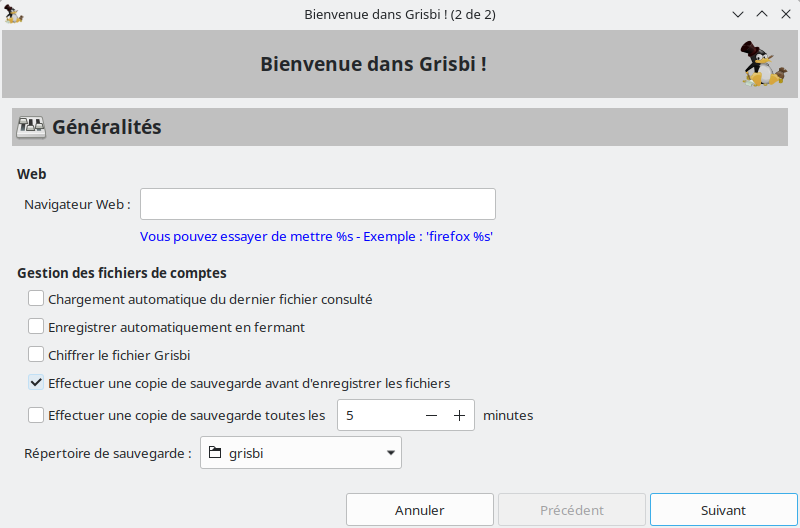
\includegraphics[width=0.98\textwidth]{image/screenshot/start_first_launch}
	\end{center}
	\caption{Initial configuration of accounts file.}
	\label{start_first_launch}
\end{figure}

It is advisable to check the options:
	\begin{itemize}
		\item Automatically load last file on startup%chargement automatique du dernier fichier consulté;
		\item Automatically save on exit;%enregistrer automatiquement en fermant;
		\item Make a backup copy before saving files (checked by default).%effectuer une copie de sauvegarde avant d'enregistrer les fichiers (coché par défaut).
	\end{itemize}
\end{enumerate}

\minisec{\textcolor{red}{\strong{Warning:}}}
The Grisbi developers recommend that you do not use the \menu{Encrypt Grisbi file} option for the following reasons:
\begin{itemize}
	\item there is no method for recovering an encrypted file whose password has been lost;
	\item For some unknown reason, using this option on Windows can render the accounts file completely unusable.
\end{itemize}  
However, if you use it, it is advisable to make regular back-ups of the unencrypted file.

\begin{enumerate}[resume]
	\item The second wizard, \enquote{Welcome to Grisbi!} (or later \enquote{New file Assistant}), which automatically follows the first, includes six steps to help you create the \indexword{account file}\index{account file}.%Le deuxième assistant \frquote{Bienvenue dans Grisbi !} (ou plus tard \frquote{Aide à la création d'un nouveau fichier de comptes}), qui suit automatiquement le premier, comprend six étapes qui vous aiderons à la création du \indexword{fichier de comptes}\index{fichier de comptes}.
	\item This is followed automatically by the third wizard, \enquote{Create a new account}, which is used to create the first account and is described in detail in section \ref{start-newfile} below.%Puis vient automatiquement le troisième assistant \frquote{Créer un nouveau compte} qui permet de créer le premier compte et qui est décrit en détail dans la section \ref{start-newfile} ci-dessous.
\end{enumerate}

At any time you can exit any wizard with the \menu{Cancel} button.

If you do not want to use the Set-up Wizard, you can open a example file instead (see the next section \ref{start-example} below).



\section{Example file\label{start-example}}


If you want to use Grisbi immediately without having to go through the full set-up, for example to get an idea of the possibilities of this program, you can download the  \file{Example\_3.0-en.gsb} file from \lang{Sourceforge.net}\footnote{\urlSourceForgeDocumentation{}} website in the folder \enquote{textsf{examples}}.

% espace avant Attention ou Note :  mm
\vspacepdf{5mm}
\textbf{Note}: in this example file, the names of the payees etc are pure invention; any similarity with a real person or business is entirely accidental.

\section{Creation of a new set of accounts\label{start-newfile}}


The first time you use Grisbi, you will need to create a first
\indexword{accounts file}\index{accounts file}. The \gls{extension} of this file will be \file{.gsb} and its name will be \file{your-file-name.gsb}.

% TODO update below

Immediately afterwards, you will need to create at least one account, and then some other accounts (current accounts, savings, credit, possibly a cash account and some transition accounts) that will contain their respective transactions.

For personal accounting, you will normally have only one account file, as this supports all the links between your different accounts. If you manage a busniess, or another personal account without a financial relationship with the first one, you will create another account file, which will have another name \file{your-second-file.gsb}. Thus \indexword{accounting entities}\index{accounting entity} will remain well separated.


% espace avant Attention ou Note : 5 mm
\vspacepdf{5mm}

\strong{Caution}: for a given reporting entity, it is necessary and important to distinguish between the  \enquote{\indexword{accounts file}\index{accounts file}} and the  \enquote{\indexword{account files}\index{account files}}:
\begin{itemize}

\item The \enquote{accounts file} you have created will have the extension \file{.gsb} and the name of \file{your-file.gsb}; it contains all the data of all the accounts created for the management of an accounting entity;

\item The \enquote{account files} are files that you may need to use or create to import or export data from one accounting application to another; these files will only contain data from one account (current or otherwise) at a time; they will have different extensions (\file{.ofx}, \file{.csv} or \file{.qif}) depending on their content; for more details, see the chapter \vref{move}, \menu{Export and import of accounts}.
\end{itemize}

% espace aprs Attention ou Note: 5 mm
\vspacepdf{5mm}
In other words, all the accounts in your household accounts are recorded in a single accounts file, and all the accounts in your business are stored in a separate accounts file; and an account in Grisbi can correspond to an account file, but only when talking about importing or exporting data.

% espace pour changement de thme
\vspacepdf{5mm}

The general procedure for creating an account file is as follows: click on the menu File - New Account File; the account file creation wizard opens, which includes six steps. In the sixth step, the assistant offers you:

\begin{itemize}
\item  create a new account, and then follow the account creation wizard, which itself includes five steps, to create the first account (because it is essential to have at least one account);
\item or to use pre existing data, then use the import wizard, which also includes five steps, to import existing account operations.
\end{itemize}

After creating this first account or importing existing account transactions, if you want to create other accounts, you will return to the end of the process of creating the account file, which will return you in both cases to the create a new account option.


% espace pour changement de thme
\vspacepdf{5mm}
To create your accounts file, click the File - New Account File menu; the detailed procedure is as follows:
enumerate
welcome window: confirm with the Forward button;

To create your accounts file, click the \menu{File - New Account File} menu: the detailed procedure is as follows:

\begin{enumerate}
\item New file assistant welcome window: confirm with the \menu{Forward} button:
\item General configuration
générale\refimage{start-file-create-img}:




\begin{figure}[htbp]
\begin{center}
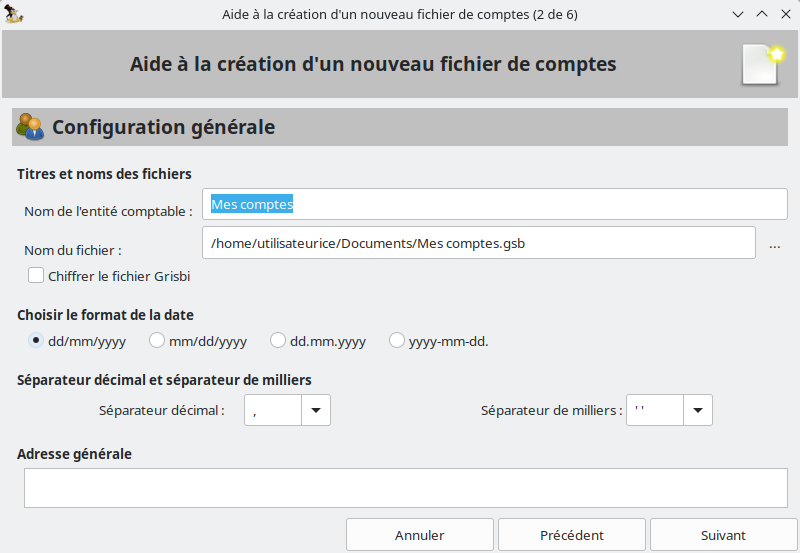
\includegraphics[scale=0.5]{image/screenshot/start_file_create}
\end{center}
\caption{General configuration of an account file}
\label{start-file-create-img}
\end{figure}



\begin{enumerate} 
 \item choose the name of the accounting entity whose accounts you are managing, for example \enquote{My accounts}, which can be chosen as the title of the Grisbi application home page,
\item enter the name of the accounts file with its complete tree; Grisbi defaults to the same name as the reporting entity, but you can change it
\item check the  \menu{Encrypt Grisbi} box if you wish \gls{to encrypt} the accounts file,
\item select the \indexword{date format}\index{date format} with one of the two buttons: dd/mm/yyyy for day/month/year, or  mm/dd/yyyy for month/day/year,
\item choose the decimal \indexword{separator}\index{separator} and the thousands from the drop-down lists,
 \item fill in the address (optional),
 \item  confirm with the  \menu{Forward} button;
\end{enumerate}

\item selection of the base \indexword{currency}\index{currency}:
\begin{enumerate} 
 \item click on the chosen currency in the list,
\item check the "include obsolete currencies" box if you also want to display old currencies,
\item confirm with the \menu{Forward} button;
\end{enumerate}

\item selection of the  \indexword{list of categories}\index{catgories !types} you will use:
\begin{enumerate} 
 \item click on your desired category, either the \menu{Standard category list} or the \menu{Empty list} \footnote{\strong{Translators Note:} Users installing the program on a system with a French Language interface will find different categories are offered including some for business users} 
\item check the \menu{Display foreign category sets} box to check if other categories are available\footnote{\strong{Translators Note:} This option is mainly for the benefit of users of a computer system with the French Language interface who will then be shown the two English categories mentioned in the previous step}
\item confirm with the \menu{Forward} button;
\end{enumerate}

\item Enter details of \indexword{banks}\index{banques !définition} holding your accounts:
\begin{enumerate} 
 \item click  \menu{Add} to define a bank; fill in the details of the bank (name, bank code, etc.), then confirm with the \menu{Add} to add the bank,
\item select a bank from the list and click the \menu{Remove} button to delete a bank, then confirm in the window that opens,
\item repeat actions a and b as many times as necessary,
\item  confirm with the \menu{Forward}  button to go to the next step, \menu{Creating a new account}:
\end{enumerate} 

\item configuration completed: the configuration of the accounts file is complete, and this window offers you to choose one of the two methods of creating your first account
compte\refimage{start-account-choice-img}:


\begin{figure}[ht]
\begin{center}
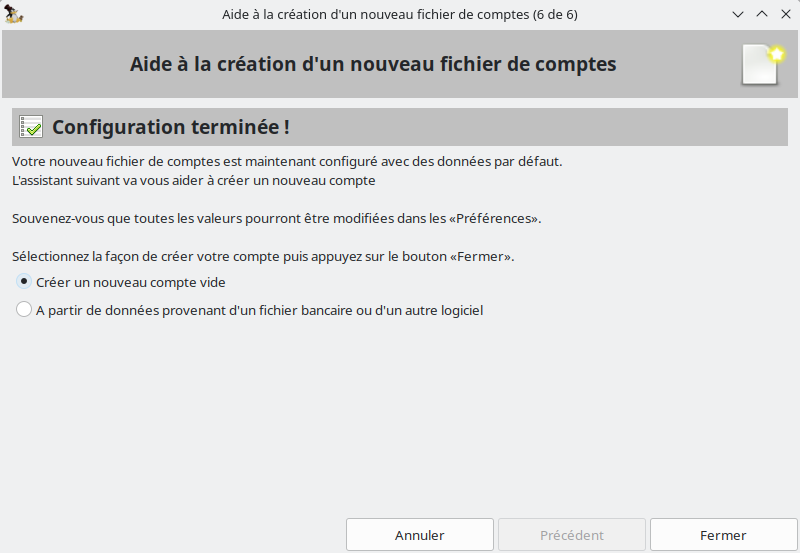
\includegraphics[scale=0.5]{image/screenshot/start_account_choice}
\end{center}
\caption{Selecting the first account}
\label{start-account-choice-img}
\end{figure}


\begin{itemize}
\item \menu{Create a new empty account}: if you check this line, then if you confirm with the \menu{Close} button, this window closes and the new account creation wizard starts. See  \vref{accounts-new}, \menu{Creating a new account},  which fully describes this procedure, then return to this page:

\item \menu{From data from a bank file or other software}: if you check this line and then confirm with the \menu{Close} button ,  this window closes and the Import Data Wizard of a file account by Grisbi starts. See the \vref{move-import-importinit} section, \menu{Importing Account Files from Another Programme into Grisbi}, which fully describes this procedure, then return to this page.
\end{itemize}
\end{enumerate}

% tiquette du paragraphe suivant, pour que les liens hypertexte dans account.tex et QIF.tex  arrivent bien dessus
\label{start-newfile-end}

\textit{\textbf{In one way or another}}, you have now created your accounts file, as well as the first account of this file.

%espace pour changement de thme
\vspacepdf{5mm}

If you want to create other accounts now, select the \menu{Edit - New Account} to create another account (see the \vref{accounts-new}, \menu{ Creating a new account} section).

%espace pour changement de thme
\vspacepdf{5mm}

Otherwise, you can start using the account you just created or the one from which you just imported the data.

% espace avant Attention ou Note : 5 mm
\vspacepdf{5mm}

\strong{Warning}: in general, it is inadvisable to have accents or spaces in the names of directories and files used by Grisbi. If so, rename them now. For example, spaces can be replaced by underscores (\underline{}).

% saut de page pour titre solidaire
\newpage


\section{Saving your accounts file\label{start-save}}

Your operations are not written as you enter them as they might be in other software; you must therefore save your account file before exiting. Do not worry, Grisbi warns you if you have not done so.

You can configure the options for saving the account file in the  \menu{ Edit - Preferences} menu, see the section \vref{setup-general-files-manage}, \menu{Managing Account Files.}.


\section{Import from other personal accounting software}

See the \vref{move-import-importinit} section to import account files from another program into Grisbi. For the moment, Grisbi supports \gls{Gnucash}, \gls{OFX}, \GLS{CSV} and \GLS{QIF} formats.



%\cleardoubleemptypage

%%%%%%%%%%%%%%%%%%%%%%%%%%%%%%%%%%%%%%%%%%%%%%%%%%%%%%%%%%%%%%%%%
% Contents: The home chapter
% $Id: grisbi-manuel-home.tex, v 0.4 2002/10/27 Daniel Cartron
% $Id: grisbi-manuel-home.tex, v 0.5.0 2004/06/01 Loic Breilloux
% $Id: grisbi-manuel-home.tex, v 0.6.0 2011/11/17 Jean-Luc Duflot
% some of its content was in menus chapter:
% $Id: grisbi-manuel-menus.tex, v 0.5.0 2004/06/01 Loic Breilloux
% $Id: grisbi-manuel-home.tex, v 0.8.9 2012/04/27 Jean-Luc Duflot
% $Id: grisbi-manuel-home.tex, v 1.0 2014/02/12 Jean-Luc Duflot
%%%%%%%%%%%%%%%%%%%%%%%%%%%%%%%%%%%%%%%%%%%%%%%%%%%%%%%%%%%%%%%%%

\chapter{Entering Grisbi\label{entrance}}%Entrée dans Grisbi

\section{Selecting a file\label{select-file}}%Sélection d'un fichier

\vspacepdf{3mm}			% vertical space = 5 mm

When you launch the application, Grisbi displays a page allowing you to get started in different ways.%Au lancement de l'application, Grisbi affiche la page qui vous permet de démarrer de différentes manières.

\vspacepdf{3mm}			% espace: 5 mm

You can display the Grisbi window in \indexword{full screen}\index{display!full screen}\index{full screen!display} by pressing the function key \key{F11}, and go back using the same key.%Vous pouvez afficher la fenêtre de Grisbi en \indexword{plein écran}\index{affichage!plein écran}\index{plein écran!affichage} par la touche de fonction \key{F11}, et revenir en arrière par la même touche.			% "!" separates the term from the subterm of the index entry

\vspacepdf{3mm}			% espace: 5 mm

\begin{figure}[htbp]			% h=here, t=top, b=bottom, p=page of float to force the figure here, not in a next page.
	\begin{center}					% image centrée
		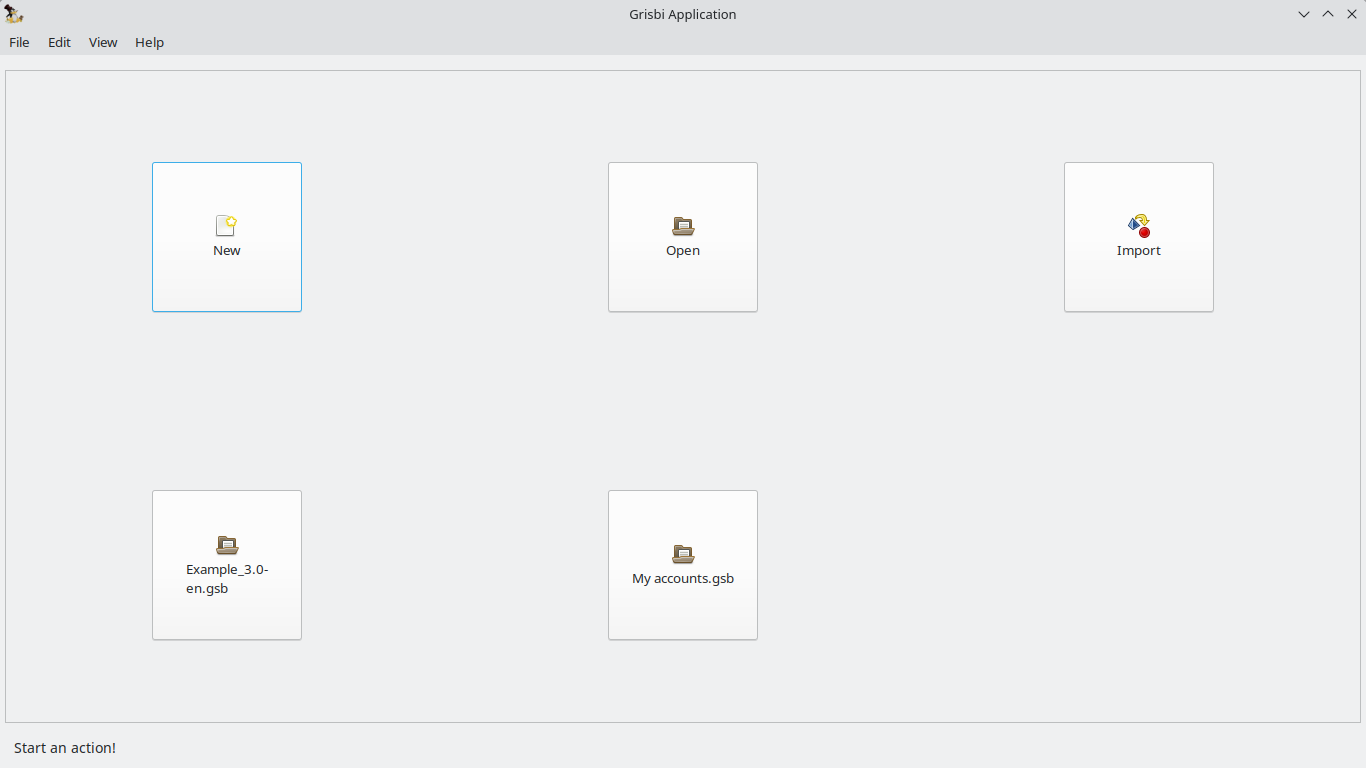
\includegraphics[width=0.95\textwidth]{image/screenshot/home_start_grisbi}		% width=95% as wide as the current text
	\end{center}
	\caption{Start-up window}%Fenêtre de démarrage}			% sous-titre/subtitle
	\label{home_start_grisbi}					% figure's ref., use for link in text with \refimage{}
\end{figure}

\vspacepdf{3mm}			% espace: 5 mm

In addition to the menu bar, this window displays a number of panels:%En plus de la barre de menu, cette fenêtre affiche plusieurs pavés:

\begin{itemize}
	\item the \enquote{New} button to launch the wizard \enquote{New file Assistant};%e pavé Nouveau, pour lancer l'assistant \frquote{Aide à la création d'un nouveau fichier de comptes};
	\item the \enquote{Open} button, to display a file manager that you can use to search for an existing accounts file on your computer;%le pavé Ouvrir, pour afficher un gestionnaire de fichier avec lequel vous pourrez chercher un fichier de comptes existant dans votre ordinateur;
	\item the \enquote{Import} button, to launch the \enquote{New file Assistant to import} wizard;%le pavé Importer, pour lancer l'assistant \enquote{Importation des opérations par Grisbi};
	\item one or more other buttons, named after account files Grisbi has already used.%un ou plusieurs autres pavés, portant le nom de fichiers de comptes que Grisbi a déjà utilisés.
\end{itemize}

\vspacepdf{5mm}	

\textbf{Note}: buttons with the names of account files that Grisbi has already used are only present if these files exist; if you want to remove them from this entry page, move them to another directory, or delete them.%les pavés portant les noms des fichiers de comptes que Grisbi a déjà utilisés ne sont présents que si ces fichiers existent; si vous voulez les enlever de cette page d'entrée, déplacez-les dans un autre répertoire, ou supprimez-les.

\vspacepdf{3mm}			% espace: 5 mm

At the bottom of the page, a banner invites you to choose an action by selecting one of these buttons.%En bas de page, un bandeau vous appelle à choisir une action en sélectionnant l'un de ces pavés.

\vspacepdf{3mm}			% espace: 5 mm

If you just want to discover the Grisbi software to get an idea of what it looks like and what it can do, you can instead use an example file like the one on the \lang{Sourceforge.net}\footnote{\urlSourceForgeDocumentation{}} site in the \enquote{\textsf{examples}} folder.%Si vous voulez juste découvrir le logiciel Grisbi pour avoir un aperçu de son aspect et de ses possibilités, vous pouvez à la place utiliser un fichier exemple comme celui présent sur le site de \lang{Sourceforge.net}\footnote{\urlSourceForgeDocumentation{}} dans le dossier \frquote{\textsf{examples}}.		% (voir la section \vref{new-example}).

\vspacepdf{5mm}			% espace: 5 mm

\textbf{Note}: by simply clicking on the downloaded example file, Grisbi will run, displaying the home window\refimage{home_3.0} directly without going through the start-up window.%en cliquant simplement sur le fichier exemple téléchargé, Grisbi s'exécutera en affichant directement la fenêtre d'accueil\refimage{home_3.0} sans passer par la fenêtre de démarrage.


\section{Homepage\label{home}}

\vspacepdf{3mm}

When an account file is opened, Grisbi displays its home page\refimage{home_3.0}.%When the application starts, Grisbi displays this
This is the start page of the programme and can be accessed at any time by clicking on the \menus{Accounts} tab.%This opening screen can be accessed at any time by clicking on the  \menus{Accounts} tab. 

\vspacepdf{3mm}

\begin{figure}[htbp]			% h=here, t=top, b=bottom, p=page of float to force the figure here, not in a next page.
	\begin{center}
		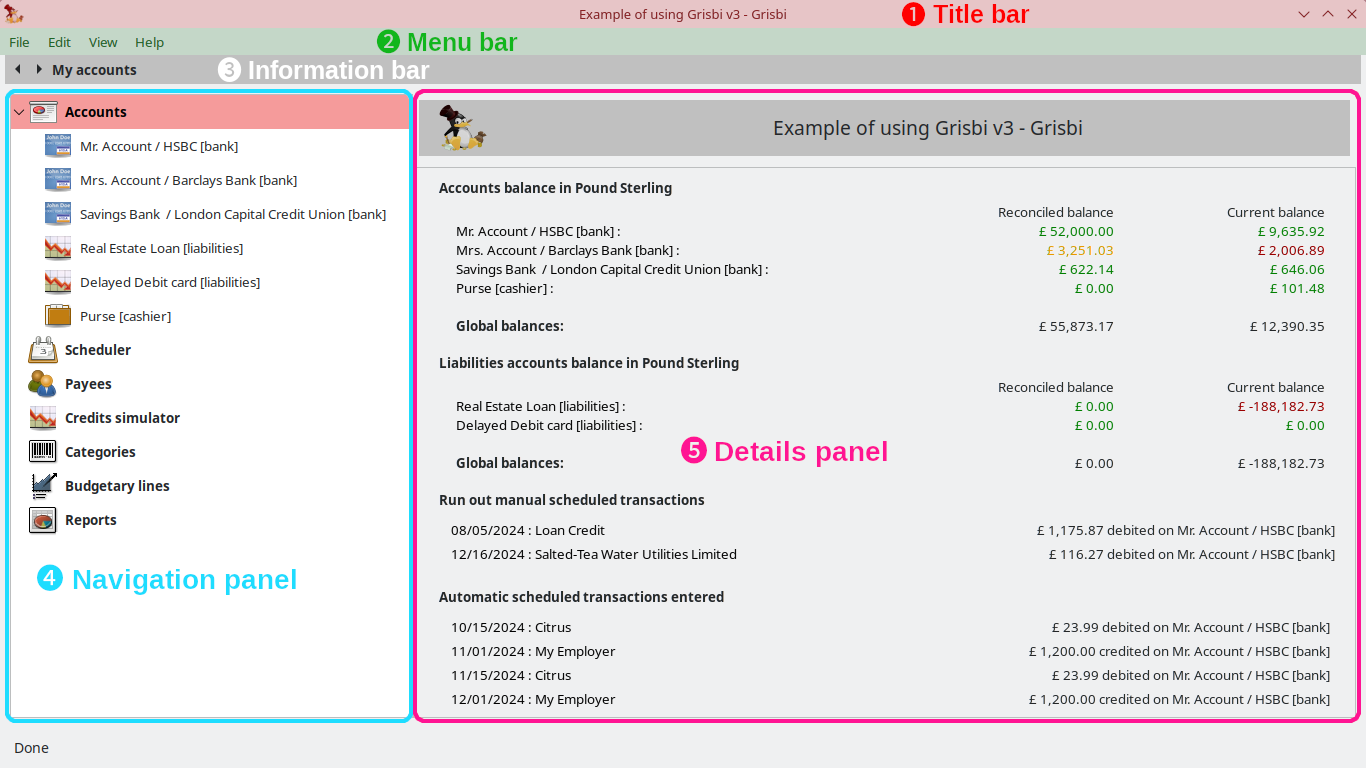
\includegraphics[width=1\textwidth]{image/screenshot/home_3.0.png}
	\end{center}
	\caption{Accounts summary page}		% sous-titre/subtitle
	\label{home_3.0}
\end{figure}

\vspacepdf{3mm}

Grisbi displays all pages in the same way: like any software, it displays:

\begin{itemize}%[\large \textcircled{\small 2}]
	\item[\large\textcircled{\small 1}] the title bar%une barre de titre;
	\item[\large\textcircled{\small 2}] the menu bar, which gives access to most of Grisbi's important functions;%une barre de menus qui donne accès à la plupart des fonctionnalités importantes de Grisbi;
\end{itemize}
as well as three specific Grisbi zones:%et aussi trois zones qui sont spécifiques à Grisbi:
\begin{itemize}%[3,4,5]
	\item[\large\textcircled{\small 3}] the information bar, under the menu bar;%la barre d'information, sous la barre de menus;
	\item[\large\textcircled{\small 4}] the navigation panel;%le panneau de navigation;
	\item[\large\textcircled{\small 5}] the details panel;le panneau des détails
\end{itemize}

\section{Information bar\label{home-synthesis}}

The information bar shows the name of the currently selected tab selected, and can display, completely to the right, certain balances relating to what is selected in the details panel.%The information bar shows the name of the current tab displayed, and can display, completely to the right, certain balances relating to what is selected in the details panel.%The information bar displays the name of the current tab displayed, and can display, to the far right, the current balance if one of the accounts is selected for display in the main screen area.

\vspacepdf{5mm}

\textbf{Note}: the information bar, displayed by default, can be hidden by unchecking a box in the preferences \vref{setup-display-toolbars}.

\vspacepdf{3mm}

To select one of the tabs displayed in the navigation panel click one or more times on one of the two small triangles on the top left of the panel.  The items displayed are: \menus{Accounts}, \menus{Scheduler}, \menus{Payees}, \menus{Credits simulator}, \menus{Categories}, \menus{Budgetary lines} and \menus{Reports}.  If the \menus{Accounts} and \menus{Reports} items have been expanded to display their sub categories these will also be displayed one by one.

\vspacepdf{5mm}

\textbf{Note}: Depending on the theme of the desktop environment or window manager you are using, these triangular symbols might be replaced by other characters such as +, -, >, <, etc.

\vspacepdf{3mm}
The content of the selection is displayed in the details panel.

\vspacepdf{3mm}
These functions can be used in place of the Navigation panel when its width is reduced to zero and you do not have direct access to it.


\section{Navigation panel\label{home-accounting}}

\begin{wrapfigure}{l}{0.33\textwidth}%50mm}
	\vspace{-\intextsep}				% space above the floating (minus intextsep=separation between float and text in text)
	\centering							% centering the floating figure in the "wrap"
	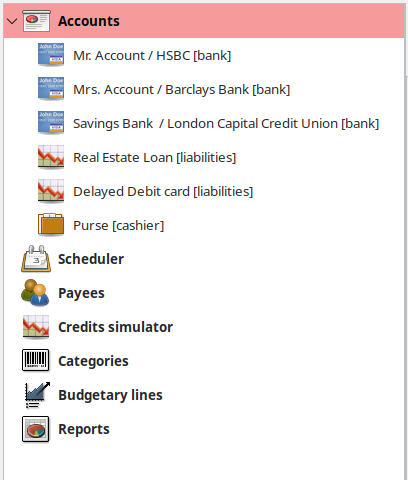
\includegraphics[width=0.28\textwidth]{image/screenshot/home_navigation}
	\vspace{-5pt}						% space between the floating and the caption below the floating
	\captionsetup{%						% for a change of options of the caption package
	format=plain,					% to avoid error message with labelsep option below, default=hang
	name=Fig.,						% rename label caption, default="Figure" (or "Table")
	justification=centering,		% centring of text and caption label 
	labelsep=newline				% define the separator between the label and the caption text
}
	\caption{Navigation panel}		% \caption is mandatory to reference a figure in lof
	\vspace{-40pt}						% space below the caption
	\label{home_navigation}
\end{wrapfigure}

The navigation panel displays in bold the list of tabs:
\begin{itemize}
	\item \menus{Accounts},
	\item \menus{Scheduler},
	\item \menus{Payees},
	\item \menus{Credits simulator},
	\item \menus{Categories},
	\item \menus{Budgetary lines},
	\item \menus{Reports}.
\end{itemize}
By clicking on the small black triangle to the left of the \menus{Accounts} or \menus{Reports} tabs,  you can scroll or roll up the list of their sub-tabs. You can change the order of tabs and sub-tabs by clicking on one of them and dragging it up or down the list.

\vspacepdf{5mm}

\textbf{Note}: Depending on the theme of the desktop environment or window manager you are using, these triangular symbols might be replaced by other characters such as +, -, >, <, etc.

\vspacepdf{3mm}

You can select one of these tabs or sub-tabs by clicking on its name. You can also move the selection in this list of tabs and sub-tabs with the \keys{Up Arrow}, \keys{Down Arrow}, \keys{Page Up} ou \keys{Page Down} keys, or with the mouse wheel (option to be checked in the preferences \vref{setup-display-toolbars}). 

\vspacepdf{3mm}
The contents of the selection are displayed in the details panel.

\vspacepdf{3mm}
You can reduce or enlarge the width of the navigation panel by clicking on the thin vertical bar between this panel and the details panel, and moving it. If the width of the window has been reduced to zero, or enlarged to the maximum of the width of the Grisbi window, the thin vertical bar may be to the left or to the right of the window.  Locate this and slide it back to the desired location.

\vspacepdf{3mm}

The \indexword{context menus}\index{context menus}, accessible by a right-click of the mouse, are available on the elements of this panel and offer the following functions:

\begin{itemize}
	\item On \menus{Accounts}:
		\begin{itemize}
			\item \menus{New account};
		\end{itemize}
	\item On any account: 
		\begin{itemize}
			\item \menus{New account},
			\item \menus{Remove this account};
		\end{itemize}
	\item On \menus{Payees}:
		\begin{itemize}
			\item \menus{New payee},
			\item \menus{Delete selected payee},
			\item \menus{Edit selected payee},
			\item \menus{Manage payees},
			\item \menus{Remove unused payees};
		\end{itemize}
	\item On \menus{Categories}: 
		\begin{itemize}
			\item \menus{New category},
			\item \menus{Delete selected category},
			\item \menus{Edit selected category},
			\item \menus{Import a file of categories (.csgb)},
			\item \menus{Export the list of categories (.csgb)}:
		\end{itemize}
	\item On \menus{Budgetary lines}:
		\begin{itemize}
			\item \menus{New budgetary line},
			\item \menus{Delete selected budgetary line},
			\item \menus{Edit selected budgetary line},
			\item \menus{Import a file of budgetary lines (.isgb)},
			\item \menus{Export the list of budgetary lines (.isgb)};
		\end{itemize}
	\item On \menus{Report}: \menus{New report};
	\item On any report: 
		\begin{itemize}
			\item \menus{New report},
			\item \menus{Remove this report}.
		\end{itemize}
\end{itemize}

\section{Details panel\label{home-details}}

The details panel displays all the details on the tabs or sub-tab selected by the Information bar or Navigation panel. This is the main work area of Grisbi.

You can reduce or enlarge its width by clicking on the thin vertical bar between this window and the navigation panel, and dragging it. If the width of the this panel has been reduced to zero or enlarged to the maximum of the width of the Grisbi window, the thin vertical bar may be to the left or to the right of the window. Locate this and slide it back to the desired location.

\begin{figure}[htbp]			% h=here, t=top, b=bottom, p=page of float to force the figure here, not in a next page.
	\begin{center}
	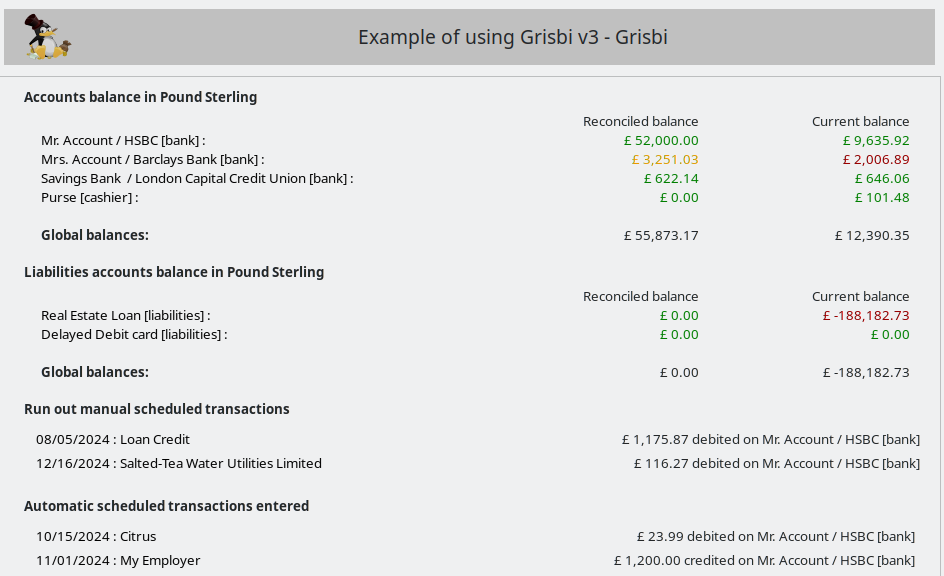
\includegraphics[width=1\textwidth]{image/screenshot/home_details.png}
	\end{center}
	\caption{Modified details panel}		% sous-titre/subtitle
	\label{home_details}
\end{figure}

\subsection{Displaying details on the home page\label{home-details-homepage}}

By selecting the \menus{Accounts} tab, the details panel displays:

\begin{itemize}
	\item to the top in a grey background banner:
	\begin{itemize}
		\item on the left, the \menus{Grisbi} icon (which can be hidden, see \vref{setup-display-logo-icon}),
		\item and on the right the \indexword{title}\index{title display!title}\index{home page} of the accounts file you currently have loaded, in the form \enquote{assigned name - Grisbi}; you can define this label, from among three possibilities, in the \menus{Edit - Preferences} menu (see the \vref{setup-display-addresses-titles} paragraph, Addresses \& titles):
		\begin{itemize}
			\item the \menus{Accounting entity} (by default): this is the name you use to identify the type of account e.g. \enquote{My Accounts} or \enquote{Business}, which you entered when the account file was created; you can edit it here in the \menus{Name of accounting entity} field; this can be useful if you manage multiple \indexword{accounting entities}\index{accounting entity}, 
			\item the \menus{Account owner name}: the name of the owner (or account manager) of the last account accessed; if the holder is not defined in the account properties, Grisbi displays the name of this account,
			\item the \menus{Filename}: this is the name of the file in the current directory, in the form  \file{name\_of\_your\_file.gsb};
		\end{itemize}
	\end{itemize}
	\item in the main light grey area below the banner:
	\begin{itemize}
		\item for each currency separately, for all accounts and \indexword{groups of accounts}\index{group of accounts}, under the label \menus{Reconciled balance} and \menus{Current balance}:
		\begin{itemize}
			\item the balance of the bank and cash accounts, the partial balance of the groups of accounts and their global balance,
			\newline
			\textbf{Note}: you can adjust the display order of the partial balances of the account groups (see the section \vref{setup-general-home-partBalance}, \menus{Partial balances of the list of accounts}),		 
			\item the balance of the liability accounts and their final balance,
			\item the balance of the asset accounts and their final balance;
		\end{itemize}
	\item the \indexword{warnings from automatically scheduled entries}\index{alert!scheduled entry} with their date, wording and amount, according to the choices made in the \menus{Edit - Preferences} menu (see the section \vref{setup-general-planned}, \menus{Scheduler}),
	\item the list of accounts whose balance has fallen below the \menus{Minimum authorized balance},
	\item the list of accounts whose balance has fallen below the \menus{Minimum desired balance}.
	\end{itemize}
\end{itemize}

\vspacepdf{5mm}

\textbf{Note}: For definitions of \menus{Minimum authorized balance} and \menus{Minimum desired balance}, see the \vref{accounts-properties}, \menus{Account Properties} section.

\vspacepdf{3mm}

The account labels are displayed in \textcolor{black}{black}: as the mouse cursor moves over the line of one of these, its colour changes to \textcolor{gray}{grey}.

A balance greater than the \menus{Minimum desired Balance} is displayed in \textcolor[RGB]{0,126,0}{green}: as the cursor moves over the line, its colour changes to \textcolor[RGB]{0,227,0}{light green}.

A balance less than the \menus{Minimum desired balance} and greater than the \menus{Minimum authorized balance} is displayed in \textcolor[RGB]{230,155,0}{orange}: as the pointer passes on its line, this color changes to \textcolor[RGB]{255,200,0}{light orange}.

A balance less than the  \menus{Minimum authorized Balance}  is displayed in \textcolor[RGB]{153,0,0}{dark red}: as the pointer passes over its line, this color changes to \textcolor{red}{red}.

When you move the mouse pointer over the line of an account, any color change indicates that if you click (right or left) with the mouse, the records contained in the highlighted account is displayed, as if the account had been selected with the information bar or navigation panel.

A partial balance can be specified for a group of accounts  If defined this is displayed in \textcolor[RGB]{40,40,255}{dark blue} (as in the figure \vref{home_details}). If it is negative, it may appear in \textcolor[RGB]{153,0,0}{dark red}, (see  \vref{setup-general-home-partBalance}, \menus{Balances partials of the list of accounts}). A partial balance line does not change color when the mouse pointer is over it, because you can not view the individual entries for of an group of accounts.

% espace pour changement de thème
\vspacepdf{3mm}
You can configure certain aspects of the display of the details panel:
\begin{itemize}
	\item in the \menus{Edit - Preferences} menu: %TODO verify sections/paragraphs with \vref{setup-xxx}
	\begin{itemize}
		\item \menus{\indexword{Generalities}\index{generalities}}:
		\begin{itemize}
			\item \menus{Various settings}, \menus{Scheduler}\index{scheduler} tab: section \vref{setup-general-planned};
			\item \menus{Main page}:
			\begin{itemize}
				\item \menus{Calculation of balance}: paragraph \vref{setup-general-home-balance},
				\item \menus{Balances partials of the list of accounts}: paragraph \vref{setup-general-home-partBalance};
			\end{itemize}
		\end{itemize}
		\item \menus{\indexword{Display}\index{display}}:
		\begin{itemize}
			\item \menus{Fonts \& Logo}\index{fonts}\index{logo}: section \vref{setup-display-logo},
			\item \menus{Addresses \& titles}\index{title}\index{addresses}: section \vref{setup-display-addresses-titles};
		\end{itemize}
	\end{itemize}
	\item in the \menus{Properties} tab of each account in the \menus{Balances} section:
	\begin{itemize}
		\item Accounts below the \menus{Minimum authorised balance}\index{balance!minimum authorised}: section \vref{accounts-properties}:
		\item Accounts below the \menus{Minimum desired Balance}\index{balance!minimum desired}: section  \vref{accounts-properties}.
	\end{itemize}
\end{itemize}

%In particular, if you find a spelling error in this page, you can correct it: see the paragraph \vref{setup-general-home-final}, \menus{?? Pluriel de final ??} !

\section{Menu bar\label{home-menus}}

As in many graphics applications, most of Grisbi's important features are accessible through the menus in the \indexword{Menu Bar}\index{menu bar}. The features are detailed below.


\subsection{\menus{File} menu\label{home-menus-file}}

This menu includes the following functions:

\vspace{3mm}
\begin{itemize}[rightmargin=.6cm]
	\item \menus{New window}: non-functional (perhaps in the future?) %TODO: to update
\end{itemize}

\noindent
\begin{minipage}{.7\linewidth}
	\begin{itemize}[rightmargin=.6cm]
	\item \menus{New account file}: creates a new Grisbi file of \gls{extension}\file{.gsb}; the current file is therefore closed and a new empty file is created with an empty account (shortcut \keys{Ctrl+N}), see the section \vref{start-newfile}; not to be confused with the creation of a new account;%\menus{Nouveau fichier de comptes}: crée un nouveau fichier Grisbi d'\gls{extension} \file{.gsb}; le fichier courant est donc fermé et un nouveau fichier vide est créé avec un compte vide (raccourci-clavier \keys{Ctrl+N}), voir la section \vref{start-newfile}; à ne pas confondre avec la création d'un nouveau compte;	 
	\item \menus{Open}: opens your file manager, allowing you to search for, select and open an account file with the \file{.gsb} \gls{extension} (shortcut \keys{Ctrl+O}).%ouvre votre gestionnaire de fichiers, permettant de rechercher, sélectionner et ouvrir un fichier de comptes d'\gls{extension} \file{.gsb} (raccourci-clavier \keys{Ctrl+O});
	\item \menus{Recently opened files}: displays a list of the last n files opened with Grisbi (only if more than one has been opened); this number is configurable in the menu \menus{Edit - Preferences}, see section \vref{setup-general-files-manage}, \menus{Account Files Management};%affiche la liste des n derniers fichiers ouverts avec Grisbi (seulement s'il y en a eu plusieurs); ce nombre est configurable dans le menu \menus{Edition - Préférences}, voir la section \vref{setup-general-files-manage}, \menus{Gestion des fichiers de compte};
	\end{itemize}
\end{minipage}
\hspace{10pt}	
\begin{minipage}{.3\linewidth}
	\vspace{-10pt}					% space above the floating (minus intextsep=separation between float and text in text)
	\centering						% centering the floating figure in the "wrap"
		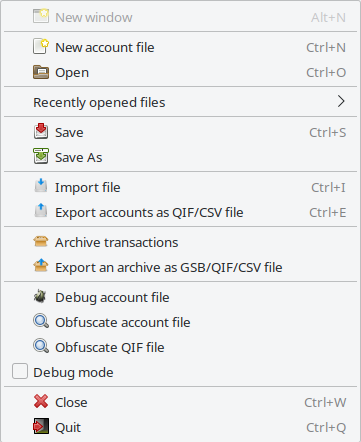
\includegraphics[width=1\textwidth]{image/screenshot/home_menubar_file}
	\vspace{-10pt}					% space between the floating and the caption below the floating
	\captionsetup{
	type=figure,%				% define "figure" or "table" type, mandatory
	name=Fig.,%					% rename label caption, default="Figure" (or "Table")
	labelsep=newline}			% define the separator between the label and the caption text
	\caption{\menus{File} menu}	% \caption is mandatory to reference a figure in lof
	%\vspace{30pt}					% space below the caption
	\label{home_menubar_file}
\end{minipage}

\begin{itemize}
	\item \menus{Save}: Saves the current account file (shortcut \keys{Ctrl+S});%\menus{Enregistrer}: enregistre le fichier de comptes en cours (raccourci-clavier \keys{Ctrl+S});
	\item \menus{Save As}: opens a file manager to save the current accounts file with the name and location of your choice; Grisbi defaults to the current directory, the name of the current accounts file, with the \file{.gsb} extension;%\menus{Enregistrer sous}: ouvre un gestionnaire de fichiers pour enregistrer le fichier de comptes en cours avec le nom et à l'emplacement de votre choix; Grisbi vous propose par défaut le répertoire courant, le nom du fichier de comptes en cours, avec l'\gls{extension} \file{.gsb};
	\item \menus{Import file}: starts the \enquote{Importing transactions into Grisbi} wizard of another software (shortcut \keys{Ctrl+I}); see \vref{move-import-importinit};%\menus{Importer un fichier}: démarre l'assistant d'importation de fichiers d'un autre logiciel (raccourci-clavier \keys{Ctrl+I}); voir la section \vref{move-import-importinit};
	\item \menus{Export accounts as \gls{QIF}/\gls{CSV} file}: starts the \enquote{Exporting Grisbi accounts} wizard (shortcut \keys{Ctrl+E}); see \vref{move-export};%\menus{Exporter vers un fichier QIF/CSV}: démarre l'assistant d'exportation de fichiers de compte (raccourci-clavier \keys{Ctrl+E}); voir la section \vref{move-export};	
	\item \menus{Archive transactions}: starts the archive creation wizard; see \vref{datamanagement-history-new};%\menus{Créer une archive}: démarre l'assistant de création d'archive; voir la section \vref{datamanagement-history-new};	
	\item \menus{Export an archive as \gls{GSB}/\gls{QIF}/\gls{CSV} file}: starts the archive export wizard; see \vref{datamanagement-history-export};%\menus{Exporter une archive vers un fichier GSB/QIF/CSV}: démarre l'assistant d'exportation d'archive; voir la section \vref{datamanagement-history-export};
	\item \menus{Debug account file}: starts the debug wizard for this file, which will help you look for inconsistencies in your account file; see \vref{maintenance-file-debug};%\menus{Déboguer le fichier de comptes}: démarre l'assistant de débogage de ce fichier, qui va vous aider à chercher des incohérences dans votre fichier de comptes; voir la section \vref{maintenance-file-debug};
	\item \menus{Obfuscate account file}: starts the wizard that produces an anonymous copy of your account file; this file can be attached to a bug report; see \vref{maintenance-file-anonymous};%\menus{Rendre anonyme le fichier de comptes}: démarre l'assistant qui produit une copie anonymée (de manière irréversible) de votre fichier de comptes; ce fichier pourra être joint à un rapport de bogue; voir la section \vref{maintenance-file-anonymous};	
	\item \menus{Obfuscate QIF file}: starts the wizard that produces an anonymous copy of this file; this file can be attached to a bug report; see \vref{maintenance-QIF-anonymous};%\menus{Rendre anonyme le fichier QIF}: démarre l'assistant qui produit une copie anonymée (de manière irréversible) de ce fichier; ce fichier pourra être joint à un rapport de bogue; voir la section \vref{maintenance-QIF-anonymous};	
	\item \menus{Debug mode}: puts Grisbi in debug mode, which creates a log file of events; see \vref{maintenance-debug-mode};%\menus{Mode de débogage}: met Grisbi en mode de débogage, qui crée un fichier-journal des évènements; voir la section \vref{maintenance-debug-mode}; 	
	\item \menus{Close}: closes the current accounts file; Grisbi offers to save it if you have not already done it (shortcut \keys{Ctrl+W});%\menus{Fermer}: ferme le fichier de comptes en cours; Grisbi vous propose de l'enregistrer si ce n'est déjà fait (raccourci-clavier \keys{Ctrl+W});
	\item \menus{Quit}: close Grisbi; Grisbi will first ask you to save the accounts file, if you have not already done so (shortcut \keys{Ctrl+Q});%\menus{Quitter}: ferme Grisbi; Grisbi vous propose auparavant d'enregistrer le fichier de comptes, si ce n'est pas déjà fait (raccourci-clavier \keys{Ctrl+Q}).
\end{itemize}


\subsection{\menus{Edit} menu\label{home-menus-edit}}

\textbf{Note}: in the \menus{Edit} menu, some entries are only active when an account or transaction is selected.
%\textbf{Note}: dans le menu Édition, certaines entrées ne sont actives que lorsqu'un compte ou une opération est sélectionné(e).

This menu includes the following functions:

\vspace{3mm}
\noindent
\begin{minipage}{.7\linewidth}
	\begin{itemize}[rightmargin=.6cm]
		\item \menus{Edit transaction}: allows a selected transaction to be rectified, see section \vref{transactions-modify}, \menus{Modification d'une opération};%TODO to translate
		%\menus{Éditer l'opération}: permet la rectification d'une opération existante, voir la section \vref{transactions-modify}, \menus{Modification d'une opération};
		\item \menus{New transaction}: allows the creation of a new transaction in an account (shortcut \keys{Ctrl+T}), see the section \vref{transactions-new}, \menus{Saisie d'une nouvelle opération};%TODO to translate
		%\menus{Nouvelle opération}: permet la création d'une nouvelle opération dans un compte (raccourci-clavier \keys{Ctrl+T}), voir la section \vref{transactions-new}, \menus{Saisie d'une nouvelle opération};
		\item \menus{Remove transaction}: deletes a selected transaction, see section \vref{transactions-delete}, \menus{Deleting a transaction};
		%\menus{Supprimer une opération}: supprime une opération existante, voir la section \vref{transactions-delete}, \menus{Suppression d'une opération};
	\end{itemize}
\end{minipage}
\hspace{10pt}	
\begin{minipage}{.3\linewidth}
	\vspace{-5pt}					% space above the floating (minus intextsep=separation between float and text in text)
	\centering						% centering the floating figure in the "wrap"
		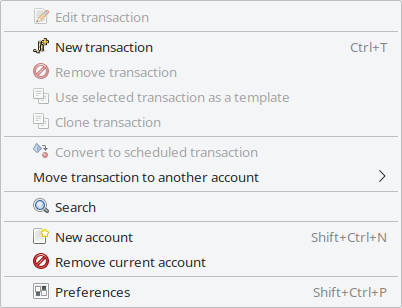
\includegraphics[width=1\textwidth]{image/screenshot/home_menubar_edit}
	\vspace{-15pt}					% space between the floating and the caption below the floating
	\captionsetup{
	type=figure,%				% define "figure" or "table" type, mandatory
	name=Fig.,%					% rename label caption, default="Figure" (or "Table")
	labelsep=newline}			% define the separator between the label and the caption text
	\caption{\menus{Edit} menu}	% \caption is mandatory to reference a figure in lof
	%\vspace{30pt}					% space below the caption
	\label{home_menubar_edit}
\end{minipage}

\begin{itemize}
	\item \menus{Use selected transaction as a template}: creates a copy of a selected transaction, with the current date entered in the transaction form, see section \vref{transactions-model}, \menus{Selecting a transaction for use as a template};
	%\menus{Utiliser l'opération sélectionnée comme modèle}: permet de créer une nouvelle opération à partir d'une opération sélectionnée, voir la section \vref{transactions-model}, \menus{Opération sélectionnée comme modèle};
	\item \menus{Clone transaction}: creates a copy identical to the selected transaction and opens the transaction form, see section \vref{transactions-duplicate}, \menus{Clone a transaction};
	%\menus{Cloner l'opération}: permet de dupliquer une opération existante, voir la section \vref{transactions-duplicate}, \menus{Clonage d'une opération};
	\item \menus{Convert to scheduled transaction}: see section \vref{transactions-schedule}, \menus{Converting a transaction to a scheduled transaction};
	%\menus{Convertir en opération planifiée}: voir la section \vref{transactions-schedule}, \menus{Conversion d'une opération en opération planifiée};
	\item \menus{Move transaction to another account}: moves the transaction to the selected account, see section \vref{transactions-move}, \menus{Moving a transaction to another account};
	%\menus{Déplacer l'opération vers un autre compte}: déplace l'opération vers le compte sélectionné, voir la section \vref{transactions-move}, \menus{Déplacement d'une opération vers un autre compte};
	\item \menus{Search}:
	\begin{itemize}
		\item opens the properties window for a report when a navigation panel tab is selected, <<<see chapter \vref{reports-creation}, \menus{Création d'un état}>>>;%TODO to modify
		%ouvre la fenêtre de propriétés d'un état quand un onglet du panneau de navigation est sélectionné, voir le chapitre \vref{reports-creation}, \menus{Création d'un état};
		\item displays the search box when an account or transaction is selected, <<<see chapter \vref{accounts-search}, \menus{alphanumeric search}>>> TO CREATE; %TODO to create
		%affiche la fenêtre de recherche quand un compte ou une opération est sélectionné, <<<voir le chapitre \vref{accounts-search}, \menus{Recherche alphanumérique}>>> A CRÉER; %TODO to create
	\end{itemize}
	\item \menus{New account}: starts the wizard for creating a new account in your Grisbi file (shortcut \keys{Shift+Ctrl+N}), see section \vref{accounts-new}, \menus{Creating a new account};
	%\menus{Nouveau compte}: démarre l'assistant de	création d'un nouveau compte dans votre fichier Grisbi (raccourci-clavier \keys{Maj \shift+Ctrl+N}), voir la section \vref{accounts-new}, \menus{Création d'un nouveau compte};
	\item \menus{Remove current account}: deletes the selected account from your Grisbi file, see section \vref{accounts-delete}, \menus{Removing the current account};
	%\menus{Supprimer le compte courant}: efface le compte sélectionné de votre fichier Grisbi, voir la section \vref{accounts-delete}, \menus{Suppression d'un compte};
	\item \menus{Preferences}: allows you to configure Grisbi (shortcut \keys{Shift \shift+Ctrl+P}); see the chapter \vref{setup}, \menus{Configuration of Grisbi}.
	%\menus{Préférences}: permet de configurer Grisbi (raccourci-clavier \keys{Maj \shift+Ctrl+P}); voir le chapitre \vref{setup}, \menus{Configuration de Grisbi}.
\end{itemize}


\subsection{\menus{View} menu\label{home-menus-display}}

\textbf{Note}: in the \menus{View} menu, entries are only active when an account is selected.

This menu includes the following functions: 

\vspace{3mm}
\noindent
\begin{minipage}{.7\linewidth}
	\begin{itemize}[rightmargin=.6cm]
	\item \menus{Show transaction form}: expands the Transaction/Scheduled form for the selected account;
	%Montrer le formulaire de saisie des opérations}: permet de développer le formulaire de saisie des opérations du compte sélectionné;
	\item \menus{Show reconciled}: displays reconciled transactions for the selected account (shortcut \keys{Alt+R});
	%Montrer les opérations rapprochées}: permet l'affichage des opérations rapprochées du compte sélectionné (raccourci-clavier \keys{Alt+R});
	\item \menus{Show lines archives}: displays the archive lines for the selected account (shortcut \keys{Alt+L});
	%Montrer les lignes d'archives}: affiche les lignes d'archives du compte sélectionné (raccourci-clavier \keys{Alt+L});
	\item \menus{Show \indexword{closed accounts}}\index{closed!account}: displays account(s) that have been closed and not deleted, see section \vref{accounts-properties}, \menus{Account properties?}; %TODO to update
	%\menus{Montrer les \indexword{comptes clos}}\index{compte!clos}: affiche le(s) compte(s) clos et non supprimé(s), voir la section \vref{accounts-properties}, \menus{Propriétés d'un compte};
	\end{itemize}
\end{minipage}
\hspace{10pt}	
\begin{minipage}{.3\linewidth}
	%\vspace{-10pt}					% space above the floating (minus intextsep=separation between float and text in text)
	\centering						% centering the floating figure in the "wrap"
		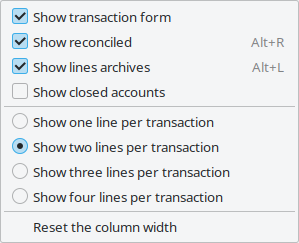
\includegraphics[width=1\textwidth]{image/screenshot/home_menubar_view}
	\vspace{-20pt}					% space between the floating and the caption below the floating
	\captionsetup{
	type=figure,%				% define "figure" or "table" type, mandatory
	name=Fig.,%					% rename label caption, default="Figure" (or "Table")
	labelsep=newline}			% define the separator between the label and the caption text
	\caption{\menus{View} Menu}		% \caption is mandatory to reference a figure in lof
	%\vspace{30pt}					% space below the caption
	\label{home_menubar_view}
\end{minipage}
\vspace{2mm}
\begin{addmargin*}[0pt]{.7cm} 	% modify margin, * : left = right, [] = obligatory argument indentation, {} = optional argument left indentation 
	The following four functions can be used to configure the display of transactions for the selected account:
	%Les quatres fonctions suivantes permettent de configurer l'affichage des opérations du compte sélectionné:
\end{addmargin*}
\vspace{-2mm}
\begin{itemize}
	\item \menus{Show one line per transaction}%Montrer une ligne par opération};
	\item \menus{Show two lines per transaction}%Montrer deux lignes par opération};
	\item \menus{Show three lines per transaction}%Montrer trois lignes par opération};
	\item \menus{Show four lines per transaction}%Montrer quatre lignes par opération};
	\vspace{2mm}
	\begin{addmargin*}[0pt]{-.35cm} 	% modify margin, * : left = right, [] = obligatory argument indentation, {} = optional argument left indentation 
	And finally, the last function in the view menu:%Et enfin la dernière fonction du menu d'affichage:
	\end{addmargin*}	
	\item \menus{Reset the column width}: allows you to reset the columns of the tranaction lists to their original width. 
	%Réinitialiser la largeur des colonnes}: permet de remettre les colonnes des listes d'opérations du compte sélectionné ou de l'échéancier à leur largeur d'origine.
\end{itemize}


\subsection{\menus{Help} menu\label{home-menus-help}}

Most of the choices in this menu give links to websites. In order for these links to work, you must have specified to Grisbi the navigation software (or Web browser) that you wish to use, in the \menus{Edit - Preferences} (see \vref{setup-general-programs}, \menus{Programmes}). The \menus{Help} menu includes the following choices:
%La plupart des choix de ce menu donnent accès à des sites Web. Pour que ces accès fonctionnent, il faut avoir indiqué à Grisbi le logiciel de navigation (ou navigateur) que vous souhaitez utiliser, dans le menu \menus{Édition - Préférences} (voir la section \vref{setup-general-programs}, \menus{Programmes}). Le menu \menus{Aide} comprend les choix suivants:

\vspace{3mm}
\noindent
\begin{minipage}{.7\linewidth}
	\begin{itemize}[rightmargin=.6cm]
		\item \menus{User's Manual}:opens your browser to the \enquote{Grisbi User Manual page} (shortcut \keys{F1}); 
		%Manuel}: ouvre votre navigateur à la page \frquote{Manuel de l'Utilisateur de Grisbi} (raccourci-clavier \keys{F1});
		\item \menus{Quick start}: opens your browser to the \enquote{Grisbi Quick Start page};
		%Démarrage rapide}: ouvre votre navigateur à la page \frquote{Démarrage Rapide de Grisbi};
		\item \menus{About}: displays the program information box: you will find details about the version, the link to Grisbi's site, the acknowledgements page (contributors to the project) and the user license;
		%À propos}: affiche la fenêtre d'information sur l'application; vous y trouverez des détails sur la version, le lien vers le site de Grisbi, les remerciements (contributeurs au projet) et la licence d'utilisation;
		\item \menus{Grisbi website}: opens your browser to the \lang{Grisbi}\footnotemark web site
		%Site Web de Grisbi}; ouvre votre navigateur à la page du site de \lang{Grisbi}\footnote{\urlGrisbi{}};
	\end{itemize}
\end{minipage}
\hspace{10pt}	
\begin{minipage}{.3\linewidth}
	%\vspace{-15pt}					% space above the floating (minus intextsep=separation between float and text in text)
	\centering						% centering the floating figure in the "wrap"
	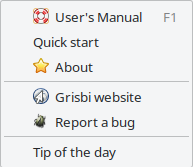
\includegraphics[width=1\textwidth]{image/screenshot/home_menubar_help}
	\vspace{-15pt}					% space between the floating and the caption below the floating
	\captionsetup{
		type=figure,%				% define "figure" or "table" type, mandatory
		name=Fig.,%					% rename label caption, default="Figure" (or "Table")
		labelsep=newline}			% define the separator between the label and the caption text
	\caption{\menus{Help} menu}	% \caption is mandatory to reference a figure in lof
	%\vspace{30pt}					% space below the caption
	\label{home_menubar_help}
\end{minipage} 
\footnotetext{\urlGrisbi{}}	% to move footnote out of minipage
\begin{itemize}
	\item \menus{Report a bug}: opens your browser to the \lang{Grisbi Bug Tracker page}\footnote{\urlBugTracker{}} to allow you to report a bug that you have discovered. You can also follow on this page the evolution of the corrections made to the reported bugs;
	%Signaler une anomalie}; ouvre votre navigateur à la page du \lang{traqueur de bogues de Grisbi}\footnote{\urlBugTracker{}} pour vous permettre de signaler un bogue que vous auriez découvert. Vous pouvez également suivre sur cette page l'évolution des corrections apportées aux bogues signalés;
	\item \menus{Tip of the day}: opens a dialog box that displays a tip of use, different each time Grisbi starts; you can successively display all the tips, and choose whether or not the display of the tip of the day when starting Grisbi. To remove or reactivate the tip of the day, see \vref{setup-display-messages-trick}, \menus{Tip of the day}.
	%Astuce du jour}; ouvre une boîte de dialogue qui affiche une astuce d'utilisation, différente à chaque démarrage de Grisbi; vous pouvez y afficher successivement toutes les astuces, et choisir ou non l'affichage de l'astuce du jour au démarrage de Grisbi. Pour activer ou supprimer l'astuce du jour, vous pouvez cocher/décocher la case \frquote{\menus{Afficher l'astuce lors du prochain démarrage}}, voir le paragraphe \vref{setup-display-messages-trick}, \menus{Astuce du jour}.
\end{itemize}


\section{Shortcut keys\label{home-shortcuts}}


Keyboard shortcuts make it easy to enter data and navigate through Grisbi's windows, avoiding the need to move and click. By using the ones corresponding to the most common manipulations for you, you improve your \indexword{ergonomics}\index{ergonomics} by limiting the important movements of your arms.
%Les raccourcis-clavier facilitent la saisie des données et la navigation dans les fenêtres de Grisbi, en évitant le recours systématique au déplacement et au clic de la souris. En utilisant ceux correspondant aux manipulations les plus courantes pour vous, vous améliorez votre \indexword{ergonomie}\index{ergonomie} en limitant les mouvements importants de vos bras.

Grisbi has a number of keyboard shortcuts, presented here according to different themes (see also  \vref{introduction-manual-conventions}, \menus{Typographical conventions in this manual}).
%Grisbi dispose d'un certain nombre de raccourcis-clavier, listés dans les préférences de Grisbi (voir \vref{{setup-display-toolbars}}), présentés ici selon différents thèmes, (voir aussi la section \vref{introduction-manual-conventions}, \menus{Conventions typographiques du présent manuel}).

\subsection{Application and files}

\begin{itemize}
	\item Create a new Grisbi file: \keys{Ctrl+N}%créer un Nouveau fichier Grisbi: \keys{Ctrl+N};
	\item Open a Grisbi file: \keys{Ctrl+O}%Ouvrir un fichier Grisbi: \keys{Ctrl+O};
	\item Add a new account to the Grisbi file: \keys{Ctrl+Shift \shift+N}%ajouter un Nouveau compte au fichier Grisbi: \keys{Ctrl+Maj \shift+N};
	\item Save the Grisbi file: \keys{Ctrl+S}%Enregistrer le fichier Grisbi: \keys{Ctrl+S};
	\item Import a file: \keys{Ctrl+I}%Importer un fichier: \keys{Ctrl+I};
	\item Export to \gls{QIF}/\gls{CSV} file: \keys{Ctrl+E}%Exporter vers un fichier \gls{QIF}/\gls{CSV}: \keys{Ctrl+E};
	\item Close the Grisbi file: \keys{Ctrl+W}%Fermer le fichier Grisbi: \keys{Ctrl+W};
	\item Close Grisbi: \keys{Ctrl+Q}%Fermer Grisbi: \keys{Ctrl+Q}.
\end{itemize}


%TODO following
\subsection{Navigation panel}

\begin{itemize}
\item Select a tab or account: \key{ Arrow Up}, \key{Arrow Down}, \key{Page Up} ou \key{Page Down}
\end{itemize}

\subsection{List of transactions and scheduled transactions}

\begin{itemize}
\item Select a transaction: \key{Enter}
\item Move selection:\key{Arrow Up} ou \key{Arrow Down}
\item New transaction:  \key{Enter} on empty line, or \key{Ctrl}\key{T}
\item Modify an transaction: \key{Enter}
\item Delete an transaction: \key{Delete}:
\item Select a transaction for a reconciliation:\key{Ctrl}\key{P}
\item Remove a reconciled transaction: \key{Ctrl}\key{R}
\item Show or hide archival lines: \key{Altl}\key{L}
\end{itemize}


\subsection{Entry form}

\begin{itemize}
\item The \key{Enter} is configurable: it can be set to either move in the input form, or to validate the entry
\item Move to the next field: \key{Tab} (depending on your configuration choice)
\item Cancel the current entry: \key{Esc}
\item Accept auto-complete: \key{Tab} or \key{Enter} (depending on your configuration choice)
\item  Euro symbol: \key{AltGr}\key{e}
\end{itemize}

\subsection{Drop down lists}

\begin{itemize}
\item Open a list: \key{Page Down} or \key{Down Arrow}
\item Move in the list: \key{Up Arrow}, \key{Down Arrow}, \key{Page Up} or \key{Page Down}
\item Validate a choice within a list: \key{Enter}
\item Currencies, ??exercises?? and methods of payment:
\begin{itemize}
\item open list: \key{Space}: 
\item move in the list: \key{Up Arrow} or \key{Down Arrow}:
\item validate the item in the list: \key{Space}.
\end{itemize}
\end{itemize}


\subsection{Dates entered on the calendar}

\begin{itemize}
\item Opens a calendar (on the date field): \key{Ctrl}\key{Enter}
\item Closes the calendar without changing the date: \key{Esc}
\item Validate the selected date: \key{Enter}
\item Next or previous day: \key{+} or \key{-}, \key{Right Arrow} or \key{Left Arrow}
\item Previous or next week: \key{Up Arrow} or \key{Down Arrow}
\item Previous or next month: \key{Page Up} or \key{Page Down}
\item First day or last day of the month: \key{Start} or \key{End}
\end{itemize}


\subsection{Dates entered on keyboard }

\begin{itemize}
\item Next or previous day: \key{+} or \key{-}
\item Previous or next week: \key{Shift} \key{+} or \key{Majuscule} \key{-}
\item Previous or next month: \key{Page Up} or \key{Page Down}
\item Previous or Next Year: \key{Shift} \key{Page Up} or \key{Shift} \key{Page Down}
\item Validate the selected date \key{Enter}
\end{itemize}


\subsection{Payees, categories, budget allocations, credit simulator, historical data and forecasts}

\begin{itemize}
\item Move selection: \key{Up Arrow}, \key{Down Arrow}, \key{Page Up} or \key{Page Down}
%Ces raccourcis ne fonctionnent plus:
%	\item afficher les sous-catégories ou sous-imputations budgétaires (sur une catégorie ou une imputation budgétaire): \key{Espace}:
%	\item afficher les opérations des sous-catégories ou sous-imputations budgétaires (sur une sous-catégorie ou une sous-imputation budgétaire): \key{Espace}.
\end{itemize}


\subsection{States and Configuration}

\begin{itemize}
\item Select another tab: \key{Up Arrow}, \key{Down Arrow}, \key{Page Up}, \key{Page Down}
\item Navigate between the tab panel and the different options in the settings panel: \key{Tab}, \key{Up Arrow}, \key{Down Arrow}, \key{Left Arrow} and \key{Right Arrow}
\end{itemize}

\subsection{Help}

\begin{itemize}
\item Open your browser on the Grisbi User Manual page \key{Ctrl}\key{H}
\end{itemize}			% TODO update screenshots and text "home", uncomment when finished
%\cleardoubleemptypage

%%%%%%%%%%%%%%%%%%%%%%%%%%%%%%%%%%%%%%%%%%%%%%%%%%%%%%%%%%%%%%%%%
% Contents: The importexport chapter
% $Id: grisbi-manuel-QIF.tex, v 0.4 2002/10/27 Daniel Cartron
% $Id: grisbi-manuel-QIF.tex, v 0.5.0 2004/06/01 Loic Breilloux
% $Id: grisbi-manuel-QIF.tex, v 0.6.0 2011/11/17 Jean-Luc Duflot
% $Id: grisbi-manuel-QIF.tex, v 0.8.9 2012/04/27 Jean-Luc Duflot
% $Id: grisbi-manuel-QIF.tex, v 1.0 2014/02/12 Jean-Luc Duflot
% $Id: grisbi-manuel-importexport.tex, v 3.0 2025/09 Dominique Brochard
%%%%%%%%%%%%%%%%%%%%%%%%%%%%%%%%%%%%%%%%%%%%%%%%%%%%%%%%%%%%%%%%%


\chapter{Importing and exporting accounts\label{importexport}}
%\chapter{Import et export de comptes\label{importexport}}

You can not directly use data that has been created by other personal accounting applications in Grisbi, and vice versa. Because these applications work differently, their data is structured differently, so you need to convert their data structure before you can use it.
%Vous ne pouvez pas utiliser directement dans Grisbi des données qui ont été créées par d'autres applications de comptabilité personnelle, et réciproquement. Comme ces applications fonctionnent différemment, leurs données sont structurées différemment: il faut donc convertir leur structure de données avant de pouvoir les utiliser. 

This conversion can not be done at once on all data, but must be done separately for each account managed by the application. To convert each of these accounts, you must first \enquote{export} them from the original application and then \enquote{import} them into the destination application.
%Cette conversion ne peut pas se faire d'un seul coup sur l'ensemble des données, mais doit se faire indépendamment pour chaque compte géré par l'application. Pour convertir chacun de ces comptes, il faut donc d'une part les \frquote{exporter} de l'application d'origine, puis les \frquote{importer} dans l'application de destination.

% espace avant Attention ou Note : 5 mm
\vspacepdf{5mm}

\Note{}: do not confuse the Grisbi file, with the \gls{extension} \file{.gsb}, which contains all the data of all the accounts created for the management of an accounting entity, and the \enquote{account files}, which are files that contain only data from one account at a time, and created only to export or import that data from one accounting application to another. These \enquote{account files} must have a \gls{file format} (or \gls{extension}) that must be compatible with the original application AND the destination application.
%\Note{}: ne pas confondre le fichier Grisbi, d'\gls{extension} \file{.gsb} et qui contient tous les comptes avec leurs données, et les fichiers de ces mêmes comptes, qui sont des fichiers ne contenant que les données d'un seul compte à la fois, et créés uniquement pour importer ou exporter ces données d'une application de comptabilité à une autre. Ces fichiers de compte doivent avoir un \gls{format de fichier} (ou une \gls{extension}) obligatoirement compatible avec l'application d'origine ET l'application de destination.


 %ne pas confondre LE \frquote{fichier de comptes} qui contient toutes les données de tous les comptes créés pour la gestion d'une entité comptable (dans Grisbi, ce fichier porte l'\gls{extension} \file{.gsb}), et LES \frquote{fichiers de compte}, qui sont des fichiers ne contenant que les données d'un seul compte à la fois, et créés uniquement pour exporter ou importer ces données d'une application de comptabilité à une autre. Ces \frquote{fichiers de compte} doivent avoir un \gls{format de fichier} (ou une extension) obligatoirement compatible avec l'application d'origine ET l'application de destination.
% espace après Attention ou Note : 5 mm
\vspacepdf{5mm}

Grisbi currently supports \gls{Gnucash}, \gls{OFX}, \gls{CSV} and \gls{QIF} personal accounting data formats.
%Grisbi supporte actuellement les formats de données de compte de comptabilité personnelle \gls{Gnucash}, \gls{OFX}, \gls{CSV} et \gls{QIF}.


\section{Importing accounts from another accounting application\label{importexport-import}}
%\section{Import de comptes d'un autre logiciel\label{importexport-import}}


If you want to use account data that has been created in another accounting application in Grisbi, you must first export each of the accounts of this application individually to a set of files, then import these same files into Grisbi.
%Si vous voulez utiliser dans Grisbi des données de comptes qui ont été créés dans une autre application de comptabilité, vous devez d'abord exporter individuellement chacun des comptes de cette application dans un fichier, puis les importer dans Grisbi grâce à ces fichiers.


\subsection{Export an account file from the other accounting application\label{importexport-import-exportinit}}
%\subsection{Export d'un compte d'un autre logiciel\label{importexport-import-exportinit}}

The first step is, in the originating personal accounting application, to export each account in a file in the chosen format. The chosen format must be compatible with the export formats supported by the original application \emph{and} compatible with import to Grisbi.
%La première étape consiste, dans l'application de comptabilité personnelle d'origine, à exporter chaque compte dans un fichier au format choisi. Le format choisi doit être compatible à l'exportation par l'application d'origine \emph{et} compatible à l'importation par Grisbi.

The export procedure is obviously different for each accounting application, so refer to its documentation. If you want to export all accounts, you will need to get as many files as you have accounts managed by the application.
%La procédure d'exportation est bien évidemment différente pour chaque logiciel, donc référez-vous à sa documentation. Si vous voulez exporter tous les comptes, vous devrez obtenir autant de fichiers que vous avez de comptes gérés par l'application.


\subsection{Importing account files from another accounting application to Grisbi\label{importexport-import-importinit}}
%\subsection{Import de fichiers de compte d'un autre logiciel dans Grisbi\label{importexport-import-importinit}}

\Note{}: Grisbi allows you to import one or more account files in one operation. Although you can import the account files one by one, it is important to import all the account files at the same time, so that Grisbi can recreate the links between the accounts, especially with regard to the transfer operations.
%\Note{}: Grisbi permet d'importer un ou plusieurs fichiers de compte au cours de la même procédure. Bien que l'on puisse importer les fichiers de compte un par un, il est important de bien importer tous les fichiers de compte simultanément, afin que Grisbi puisse recréer les liens entre les comptes, particulièrement en ce qui concerne les opérations de virement.
% espace après Attention ou Note : 5 mm
\vspacepdf{5mm}

For more information on the \indexword{account types}\index{account types} that Grisbi can manage, see the \vref{accounts-type}, \menus{Grisbi account types} section.
%Pour plus de renseignements sur les \indexword{types de compte}\index{types de compte} que Grisbi sait gérer, voir la section \vref{accounts-type}, \menus{Types de comptes de Grisbi}.

The import can be configured in the menu \menus{Edit - Preferences} (see section \vref{setup-general-import-files}), \menus{Files import} tab.
%L'import est paramétrable dans le menu \menus{Édition - Préférences} (voir la section \vref{setup-general-importLinks}, onglet \menus{Importation des fichiers}).

You can define which date will be used for assigning a financial year to each imported operation, see \vref{setup-general-import-financialyear}, \menus{Definition of Financial Year}.
%Vous pouvez définir quelle date sera utilisée pour l'attribution d'un exercice à chaque opération importée, voir le paragraphe \vref{setup-general-import-financialyear}, \menus{Définition de l'exercice}.

Grisbi also allows you to establish an association between a string of characters in this file and a payee. For example, all labels containing \enquote{rent} may be associated with a payee that represents your landlord. This must be configured in the \menus{Edit - Preferences} menu (see the \vref{setup-general-importlinks} section), \menus{Associations for import} tab.
%Grisbi vous permet aussi d'établir une association entre une chaîne de caractères de ce fichier et un tiers. Par exemple, tous les libellés contenant \frquote{loyer} peuvent être associés à un tiers qui représente votre propriétaire. Cela doit être configuré dans le menu \menus{Édition - Préférences} (voir la section \vref{setup-general-importLinks}, onglet \menus{Associations pour l'importation}).

% espace pour changement de thème
\vspacepdf{5mm}
In the Grisbi \menus{File} menu, choose the option \menus{Import file} (or use the shortcut \keys{Ctrl+I}), which opens the import wizard window. The import of the account files takes place in five steps, to which one step must be added for each additional account:
%Dans le menu \menus{Fichier} de Grisbi, choisissez l'option \menus{Importer un fichier} (ou utilisez le raccourci-clavier \keys{Ctrl+I}), ce qui ouvre la fenêtre de l'assistant d'importation. L'importation d'un seul fichier de compte se déroule en cinq étapes, auxquelles il faudra rajouter une étape par compte supplémentaire:

\begin{enumerate}
	\item Launches the import assistant (step 1/5): confirm with the \menus{Forward} button;
	%Accueil de l'assistant d'importation (étape 1/5): validez avec le bouton \menus{Suivant};
	\item Selection of the account files to import (step 2/5) \refimage{importexport-import-files-select-img}:
	%Sélection des fichiers de compte à importer (étape 2/5) \refimage{importexport-import-files-select-img}:	
		\begin{enumerate}
			\item click the button \menus{Add file to import...} button : a file manager window opens;
			%cliquez sur le bouton \menus{Ajouter un ou des fichiers...}: une fenêtre de gestionnaire de fichiers s'ouvre;
			\begin{figure}[htbp]
				\raggedleft
				%\begin{flushleft}
					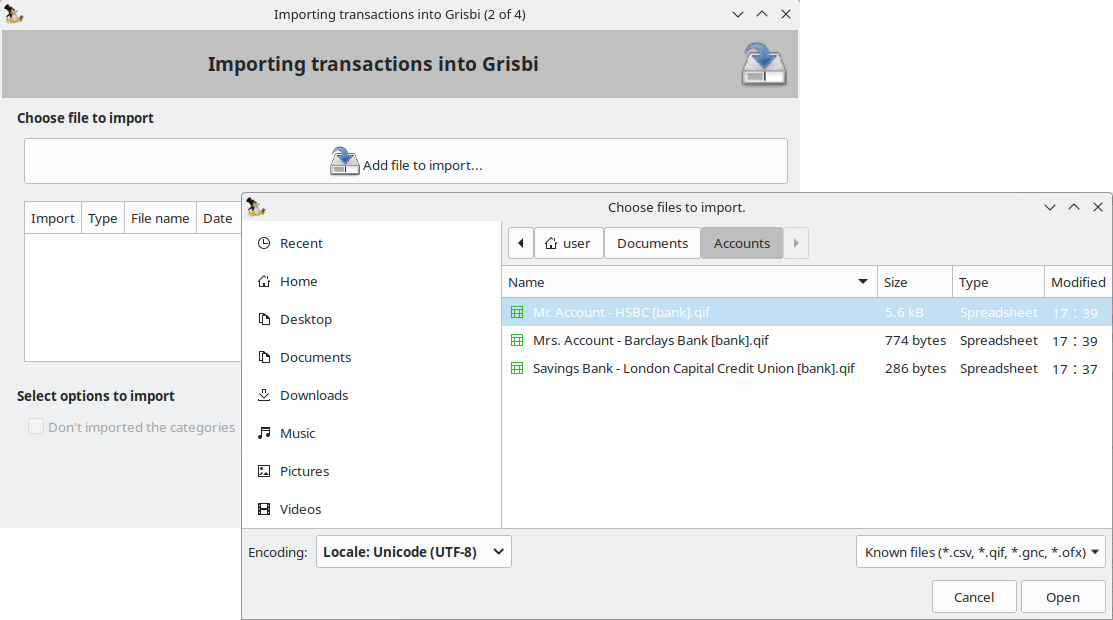
\includegraphics[width=.95\textwidth]{image/screenshot/importexport_import_files_select}
				%\end{flushleft}
				\caption{Selecting accounts to import}%Sélection des comptes à importer}
				\label{importexport-import-files-select-img}
			\end{figure}
			\item look for the directory where these account files are,
			%cherchez le répertoire où se trouvent ce ou ces fichiers de compte;
			\item select one or more account files (with the combination \keys{Ctrl+Left-Click} and \keys{Shift+Left-Click}); you can also change the \gls{locale} (\gls{character encoding}) of the files to import from the \menus{Encoding} drop-down menu,
			%sélectionnez un ou plusieurs fichiers de compte (avec la combinaison \keys{Ctrl+Clic Gauche} et \keys{Maj \shift+Clic gauche}); vous pouvez aussi changer la \gls{locale} (\gls{encodage des caracteres}) des fichiers à importer dans le menu déroulant \menus{Codage};
			\item validate the window with the \menus{Open} button to return to the account file selection window;
			%validez avec le bouton \menus{Ouvrir} pour revenir à la fenêtre de sélection des fichiers de compte;
			\item you can choose not to import categories by ticking the appropriate option. When importing a \gls{CSV} file, a new window allows you to choose the import settings \refimage{importexport-import-CSV-setup-img}:
			%vous pouvez choisir de ne pas importer les catégories en cochant l'option adéquate. Dans le cas d'import d'un fichier \gls{CSV}, une nouvelle fenêtre vous permet de choisir les paramètres d'import \refimage{importexport-import-CSV-setup-img}:
				\begin{itemize}[label=\textopenbullet]
					\begin{figure}[htbp]
						\raggedleft
						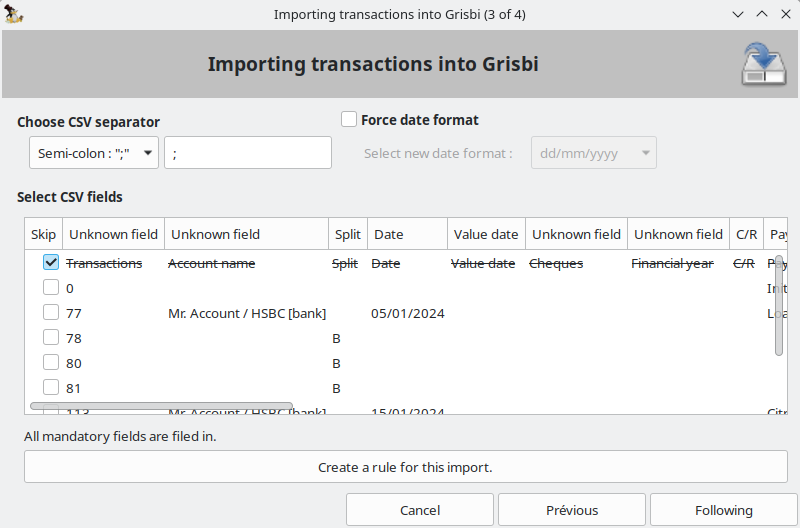
\includegraphics[width=.95\textwidth]{image/screenshot/importexport_import_CSV_setup}
						\caption{Configuring the import of a CSV file}%Paramétrage de l'import d'un fichier CSV}
						\label{importexport-import-CSV-setup-img}
					\end{figure}
					\item \textbf{Choose CSV separator}: the separator between data can be selected from the drop-down list in the left-hand window and is displayed in the right-hand window, where you can also modify it. 
					%\textbfChoisissez le séparateur CSV}: le séparateur entre les données peut être sélectionné dans la liste déroulante de la fenêtre de gauche et s'affiche dans la fenêtre de droite, où vous pourrez aussi le modifier;
					\item \textbf{Force date format}: The date format can be forced by ticking the appropriate box and selecting it from the drop-down list.
					%\textbf{Forcer le format de la date}: le format de date peut être forcé en cochant la case idoine et en le sélectionnant dans la liste déroulante;
					\item \textbf{Select CSV fields}: you can tick the data lines that \textit{will not be} imported;
					%\textbf{Sélectionnez les champs}: vous pourrez cocher les lignes de données qui \textit{ne seront pas} importées;
					\item The \enquote{Create a rule for this import.} button (at the bottom) allows you to create an import rule that you will need to name in order to validate it. You will find it in the account toolbar (see \vref{transactions-functions}).
					%le bouton \frquote{Créer une règle pour cet import.} (en bas) permet de créer une règle d'import que vous devrez nommer pour la valider. Vous la retrouverez dans la barre d'outils du compte (voir \vref{transactions-functions}).
				\end{itemize}
			\item when the desired files are checked, you can validate the selection with the \menus{Forward} button;
			%si les comptes choisis sont bien cochés, vous pouvez valider par le bouton \menus{Suivant};
		\end{enumerate}
	\item Complete the import of the account files (step 3/5): if everything went well, this window gives the list of the account files which will be imported; continue the import by confirming with the \menus{Forward} button;
	%Fin de la préparation de l'importation des fichiers de compte (étape 3/5): si tout s'est bien passé, cette fenêtre donne la liste des fichiers de compte qui seront importés; continuez l'importation en validant par le bouton \menus{Suivant};
	
	\item Creating and configuring each account imported into Grisbi (step 4): you can review each account and choose the following actions \refimage{importexport-import-files-setup-img}:
	%Création et paramétrage de chaque compte importé dans Grisbi (étape 4): vous pouvez passer en revue chaque compte et y choisir les actions suivantes \refimage{importexport-import-files-setup-img}:
	\begin{figure}[htbp]
		\begin{center}
		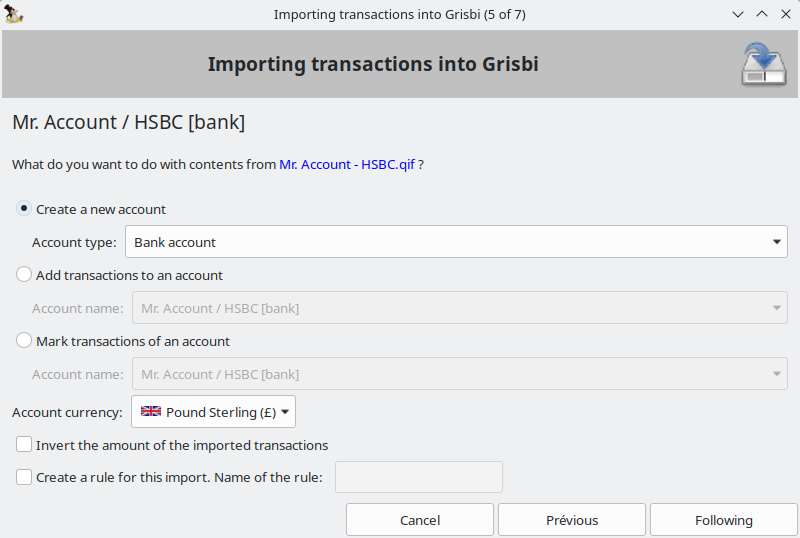
\includegraphics[width=0.95\textwidth]{image/screenshot/importexport_import_files_setup}
		\end{center}
		\caption{Configuration of each imported account}%Paramétrage de chaque compte importé
		\label{importexport-import-files-setup-img}
	\end{figure}
		\begin{itemize}
			\item \menus{Create a new account}:%Créer un nouveau compte
			this will add the selected file as a new account in your Grisbi file. The drop-down menu \menus{Account type} below will allow you to change the account type.
			% cela ajoutera le fichier sélectionné comme nouveau compte dans votre fichier Grisbi. Le menu déroulant \menus{Type de compte}, en dessous, vous permettra de modifier le type de compte;
			\item \menus{Add transactions to an account}:%Ajouter des opérations à un compte}:
			%TODO: FOLLOWING
			if scheduled operations are found within the specified time interval, a specific window opens to ask what you want to do with them: either merge these scheduled operations with the corresponding imported operations, or add the imported operations in addition to them (see the section \vref{setup-general-import-parameters}, \menus{Import settings}). The \menus{Account name} drop-down menu below will allow you to select the account to which the transactions will be added.
			% si des opérations planifiées sont trouvées dans l'intervalle de temps spécifié, une fenêtre spécifique s'ouvre pour savoir ce que vous voulez en faire: soit fusionner ces opérations planifiées avec les opérations importées correspondantes, soit ajouter les opérations importées en sus de celles-là (voir la section \vref{setup-general-import-parameters}, \menus{Paramètres pour l'import}). Le menu déroulant \menus{Nom du compte}, en dessous, vous permettra de sélectionner le compte auquel seront ajoutées les opérations;
			\item
			%\menus{Marquer les opérations d'un compte}: cela marquera les opérations avec un \frquote{T} dans la colonne \frquote{P/R} (\vref{transactions-list-fields}) du compte concerné. Si des \indexword{opérations orphelines}\index{opération!orpheline} sont trouvées, une fenêtre s'ouvrira en fin d'import pour savoir ce que vous voulez en faire: soit les ajouter, soit les ignorer. Le menu déroulant \menus{Nom du compte}, en dessous, vous permettra de sélectionner le compte dans lequel les opérations seront marquées;
			\item définir la devise du compte (ou bien en créer une nouvelle);
			\item \menus{Inverser le montant de l'opération importée}: utile pour les comptes de carte bancaire de la Banque Postale, par exemple;
			\item \menus{Créer une règle pour cet import}: permet de définir une règle d'import rapide si le fichier est au format \gls{QIF}, \gls{Gnucash} ou \gls{OFX} et uniquement si vous ajoutez ou marquez des opérations à un compte. Cette règle est spécifique à chaque compte et devra être nommée pour être validée. Vous pourrez la retrouver dans la barre d'outils du compte (voir \vref{transactions-functions});
			\item quand tout est correct, validez l'importation par le bouton \menus{Suivant};
		\end{itemize}
	\item Validation de la fin de l'importation: valider par le bouton \menus{Fermer}.
\end{enumerate}

Si, et seulement si, vous venez de créer votre fichier Grisbi juste avant cette importation de données de comptes, revenez à la fin de la section \vref{start-newfile-end}, \menus{Création d'un nouveau fichier de comptes}. Allez juste après la fin de la procédure de création du fichier de comptes, au paragraphe commençant par \textbf{\emph{D'une manière ou d'une autre\ldots{ }}}, ce qui vous proposera de créer tout de suite d'autres comptes.

%espace pour changement de thème
\vspacepdf{5mm}
Sinon, vous pouvez commencer à utiliser le compte que vous venez de créer.


\section{Export de comptes à partir de Grisbi\label{importexport-export}}


Si vous voulez utiliser, dans une autre application de comptabilité, des données de compte qui ont été créées par Grisbi, vous devez d'abord exporter ces données dans des fichiers, puis les importer dans l'autre application grâce à ces fichiers. Le format de fichier choisi doit être compatible à l'exportation par Grisbi \emph{et} compatible à l'importation par l'application de destination.
 
Dans le menu \menus{Fichier}, choisissez l'option \menus{Exporter vers un fichier QIF/CSV}  (ou utilisez le raccourci-clavier \keys{Ctrl+E}) qui ouvre l'assistant Export des comptes. L'exportation des comptes comporte à minima quatre étapes:

\begin{enumerate}
	\item Accueil de l'assistant (étape 1/3): cette fenêtre indique que, comme les formats de fichier \gls{QIF} et \gls{CSV} ne supportent pas les devises, toutes les opérations seront converties dans la devise de leur compte respectif; validez par le bouton \menus{Suivant};
	\item Sélection des comptes et des options \refimage{importexport-export-img}:
		\begin{figure}[htbp]
			\begin{center}
				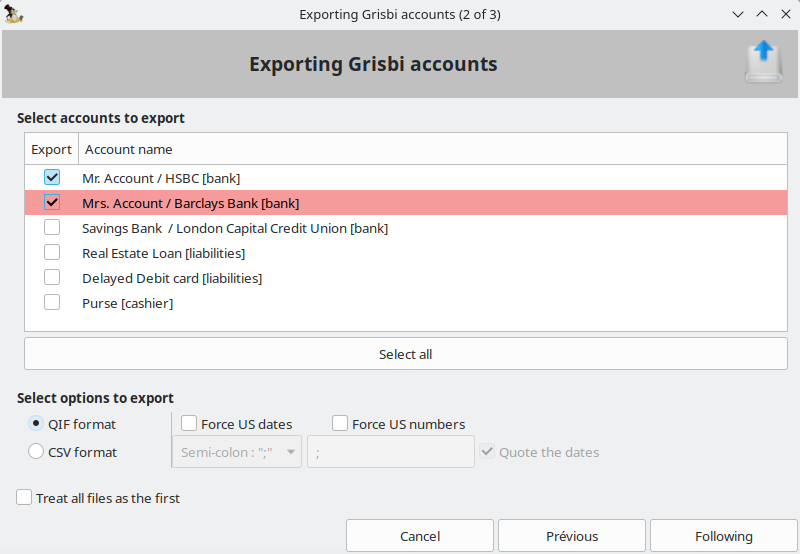
\includegraphics[width=0.95\textwidth]{image/screenshot/importexport_export}
			\end{center}
			\caption{Export des comptes}
			\label{importexport-export-img}
		\end{figure}
		\begin{itemize}
			\item \textbf{Sélectionner les comptes à exporter} (étape 2/3): cliquez sur la ou les cases correspondantes à chaque compte à exporter ou sur le bouton \menus{Sélectionner tout};
			\item \textbf{Sélectionner les options pour l'export}:
			\begin{itemize}
					\item \menus{Format QIF}: exporte le ou les comptes cochés au format \gls{QIF}; en plus l'option:
						\begin{itemize}
							\item
							%\menus{Force les dates au format US}: enregistre la date au format \frquote{mois/jour/année} (mm/dd/yyyy),
							\item
							%\menus{Force les nombres au format US}: utilise le point \frquote{.} comme séparateur de décimale et la virgule \frquote{,} comme séparateur des milliers;
						\end{itemize}
					\item \menus{Format CSV}: exporte le ou les comptes cochés au format \gls{CSV}; en plus des options disponibles au format QIF (ci-dessus):
						\begin{itemize}
							\item le séparateur entre les données peut être sélectionné dans la liste déroulante de la fenêtre de gauche et s'affiche dans la fenêtre de droite, où vous pourrez aussi le modifier;
							\item \menus{Citer les dates}: si cochée (par défaut), les dates seront mises entre guillemets, comme les autres données;
						\end{itemize}
			\end{itemize}
			\item \menus{Traiter tous les fichiers comme le premier}: ???;
			 validez par le bouton \menus{Suivant};
		\end{itemize}
	\item pour chaque compte, définissez le nom du fichier, le répertoire de destination et le format d'exportation, puis validez par le bouton \menus{Suivant}
	\item la fenêtre de fin de l'exportation s'affiche; validez par le bouton \menus{Fermer}.
\end{enumerate}

\Attention{}: d'une manière générale, il est déconseillé d'avoir des accents ou des espaces dans les noms des répertoires et fichiers utilisés par Grisbi. Si c'est le cas, renommez-les maintenant. Par exemple, les espaces peuvent être remplacées par des tirets bas (\_).			% TODO update screenshots and text "QIF", uncomment when finished
%\cleardoubleemptypage

%\include{07-grisbi-manuel-datamanagement-en}	% TODO update screenshots and text "datamanagement", uncomment when finished
%\cleardoubleemptypage

%\include{08-grisbi-manuel-accounts-en}		% TODO update screenshots and text "accounts", uncomment when finished
%\cleardoubleemptypage

%\include{09-grisbi-manuel-transactions-en}	% TODO update screenshots and text "transactions", uncomment when finished
%\cleardoubleemptypage

%\include{10-grisbi-manuel-reconciliation-en}	% TODO update screenshots and text "reconciliation", uncomment when finished
%\cleardoubleemptypage

%\include{11-grisbi-manuel-planned-en}		% TODO update screenshots and text "planned", uncomment when finished
%\cleardoubleemptypage

%\include{12-grisbi-manuel-search-en}			% TODO update screenshots and text "search", uncomment when finished
%\cleardoubleemptypage

%\include{13-grisbi-manuel-third-en}			% TODO update screenshots and text "third", uncomment when finished
%\cleardoubleemptypage

%\include{14-grisbi-manuel-categories-en}		% TODO update screenshots and text "categories", uncomment when finished
%\cleardoubleemptypage

%\include{15-grisbi-manuel-budgetlines-en}	% TODO update screenshots and text "budgetlines", uncomment when finished
%\cleardoubleemptypage

%\include{16-grisbi-manuel-financialyear-en}	% TODO update screenshots and text "financialyear", uncomment when finished
%\cleardoubleemptypage

%\include{17-grisbi-manuel-credit-en}			% TODO update screenshots and text "credit", uncomment when finished
%\cleardoubleemptypage

%\include{18-grisbi-manuel-budget-en}			% TODO update screenshots and text "budget", uncomment when finished
%\cleardoubleemptypage

%\include{19-grisbi-manuel-bankcardmanagement-en}	% TODO update screenshots and text "bankcardmanagement", uncomment when finished
%\cleardoubleemptypage

%\include{20-grisbi-manuel-association}		% fr version only
%\cleardoubleemptypage

%\include{21-grisbi-manuel-reports-en}			% TODO update screenshots and text "reports", uncomment when finished
%\cleardoubleemptypage

%\include{22-grisbi-manuel-reports-creation-en}	% TODO update screenshots and text "reports-creation", uncomment when finished
%\cleardoubleemptypage

%\include{23-grisbi-manuel-setup-en}				% TODO update screenshots and text "setup", uncomment when finished
%\cleardoubleemptypage

%\include{24-grisbi-manuel-maintenance-en}		% TODO update screenshots and text "maintenance", uncomment when finished
%\cleardoubleemptypage



%% Files editors not used anymore, so useless 
%%\include{grisbi-manuel-todo}
%%\cleardoubleemptypage
%
%% Files editors not used anymore, so useless 
%%\include{grisbi-manuel-problems}
%%\cleardoubleemptypage
%
%% Useless so don't include it
%%\include{grisbi-manuel-XML}
%
%% Useless so don't include it
%%\include{grisbi-manuel-FDL}


% Prints the index
\printindex


% Displays a note at the beginning of the glossary
\renewcommand{\glossarypreamble}{\textbf{Note}: most of the definitions in this glossary are taken from articles of the same name in the free, collaborative encyclopaedia \lang{Wikipédia}
\footnote{\urlWikipedia{}}. Although these texts have been modified and adapted to the specific context of this glossary, the author would like to thank Wikipedia for providing these references.\newline}


% Prints the glossary
% For pdf only; redefined in hva/macros.hva by an empty command in html
\printglossaries


\end{document}



